\documentclass[]{final_report}
\usepackage{graphicx}
\usepackage{hyperref}


%%%%%%%%%%%%%%%%%%%%%%
%%% Input project details
\def\studentname{Luke Sell}
\def\reportyear{2019}
\def\projecttitle{Playing Games and Solving Puzzles Using AI}
\def\supervisorname{Iddo Tzameret}
\def\degree{BSc (Hons) in Computer Science}
\def\fullOrHalfUnit{Full Unit} % indicate if you are doing the project as a Full Unit or Half Unit
\def\finalOrInterim{Plan} % indicate if this document is your Final Report or Interim Report

\begin{document}

\maketitle

%%%%%%%%%%%%%%%%%%%%%%
%%% Declaration

\chapter*{Declaration}

This report has been prepared on the basis of my own work. Where other published and unpublished source materials have been used, these have been acknowledged.

\vskip3em

Word Count: N/A

\vskip3em

Student Name: \studentname

\vskip3em

Date of Submission: 05/10/2019

\vskip3em

Signature: l.sell

\newpage

%%%%%%%%%%%%%%%%%%%%%%
%%% Table of Contents
\tableofcontents\pdfbookmark[0]{Table of Contents}{toc}\newpage

%%%%%%%%%%%%%%%%%%%%%%
%%% Your Abstract here

\chapter*{Abstract}
\addcontentsline{toc}{chapter}{Abstract}

\section*{Introduction and Background}
\addcontentsline{toc}{section}{Introduction and Background}

Sudoku is a logical puzzle where the goal is to fill an incomplete grid with numbers so that each row, column and square has all numbers up to the size of that grid. These simple rules allow Sudoku puzzles to be seen as a Constraint Satisfaction problem and thus they can be generated and solved significantly quicker by Artificial Intelligence using Constraint Satisfaction algorithms than by people.

To produce an incomplete Sudoku puzzle, a generator is required so that numbers are placed in a grid, where the amount of numbers given relates to the difficulty of that puzzle, in such a way that there is only one solution. To prove that a generated Sudoku puzzle not only has a solution, but a unique one, a solver is required to complete the puzzle and find this solution. It would also be useful to see and modify the Sudoku puzzle on a computer, so that the user of that application can solve the puzzle themselves.

\section*{Aims and Objectives}
\addcontentsline{toc}{section}{Aims and Objectives}

This project aims to use Artificial Intelligence to solve the puzzle Sudoku, it will use Backtracking to allow the AI to search for a solution to solve puzzles of any difficulty in a reasonable time, with the help of efficient algorithms, such as pruning. To allow for a puzzle to be solved using AI, a solvable puzzle must first be generated, this involves generating a random completed Sudoku grid and then removing numbers while making sure there is still only one solution to the puzzle.

This will also involve the creation of a simple GUI to display the incomplete puzzle and its solution, so that it can be viewed by a human user, as well as allowing the user to modify settings for the generation of that puzzle, and other settings relating to the displaying of the GUI. The application must also allow a human user to enter and remove numbers, and receive feedback from the application in the form of hints to possible partial solutions, warnings of mistakes and highlighting the selected rows/columns/squares, so that they can attempt to solve it themselves.

As an extension the application must also be able to save and load these puzzles at any stage of completion so that the user can continue after exiting and restarting the application. The same AI could also be adapted to solve other similar Constraint Satisfaction puzzles if there is time.

\newpage
\section*{Overview of Early Deliverables}
\addcontentsline{toc}{section}{Overview of Early Deliverables}

\subsection*{Proof of Concept Programs}

A Main Menu GUI for the Sudoku program will be created using C++ and the framework SDL 2.0 using~\cite{MITCHELL:2013}, this will involve setting up the GUI window in the main method to display the screen, with buttons that link to other screens that will be completed later.

The Data Structures used by the Sudoku program will be a Matrix to store the current Sudoku grid, and a priority queue that will be used by the AI solver in the backtrack search algorithm. The Relevant wrapper classes and the entries they store will need to be created and used by the Application.

The Eight Queens problem will involve using the existing GUI and extending it to display the Chess Board, the initial positions of the Queens will be hard coded, and the program will used a backtracking search with minimal conflicts checking to find the solution quickly and efficiently using~\cite{TSANG:1993}.

An inefficient Sudoku solver will be created to solve a Sudoku puzzle of easy difficulty, this will involve using a backtracking search to attempt to fill the partially completed grid with possible numbers until a valid solution is found, minimal conflicts can be used here to make the program more efficient, as well as backjumping and pruning if possible.

\subsection*{Reports}

A report on the Design Patterns that can be used within the AI searching algorithm and other parts of the program will be written, this will involve researching Design Patterns such as Adapter/Facade, Bridge and other Behavioural Design Patterns using~\cite{GAMMA:1995}, this will then be used to refactor the program code.

A report on Backtracking searching and recursion will be written to help design the AI solving algorithm for the Sudoku puzzle, this will cover topics like value ordering and backjumping to make the algorithm more efficient, as well as example code that can be used to better understand how the AI would solve the Sudoku puzzle.

A report on Constraint Satisfaction and Consistency techniques will be written as Sudoku can be modelled in this way, by researching CSP algorithms and techniques such as K consistency and arc/node consistency an efficient AI solving algorithm can be design to find a solution to Sudoku puzzles of any difficulty very quickly.

A report will be written on the solving techniques used by human solvers to see if this can influence the design of the AI solving algorithm, as human solving behaviour is similar to that of CSP algorithms this could allow for an algorithm to be designed that can estimate the difficulty of solving the puzzle for a person.

A report will be written on the Design of the User Interface and User Experience while using the application, this will involve drawing mock up UI designs to test different ways to display the Sudoku puzzle, this will be helpful for creating the actual application so that it is easily usable for a person to attempt to solve Sudoku puzzles and use the AI solver to find the solution to that puzzle.

A report will be written on the Complexity and Hardness of the Sudoku puzzle and the solving algorithm, this will involve using Big O Notation to find the scaling term to see how the algorithm scales with increasingly grid sizes and difficulty, and will be useful in designing more efficient algorithms that find the solution quicker so that the AI solver can be used for a wider range of grid sizes and more difficult puzzles.

\section*{Overview of Final Deliverables}
\addcontentsline{toc}{section}{Overview of Final Deliverables}

\subsection*{The Program}

The Application will also generate Sudoku puzzles to be solved by a person of the AI solving algorithm, this will involve first filling in an empty grid until it is complete, at the same time as making sure that there is one solution, so that invalid Sudoku puzzles are not generated, and then randomly removing numbers that do not create extra solutions until the smallest possible puzzle has been generated.

The Application will also be able to save and load puzzles so that a person attempting to solve the Sudoku puzzle can continue after exiting and restarting the Application, this will involve converting the Matrix grid of numbers into a format that can be written to and read from a save file, this will require the creation of a parser to correctly read the stored text and create entries to be inserted into the Matrix object.

\subsection*{The Report}

The report will also include description of Software Engineering Processes used while coding, this will involve conforming to googles checkstyle, using GitHub correctly as a Version Control System, writing tests for written code and using Design Patterns, it will also include the use of backlogs and task allocation boards like Trello or GitHubs integrated Project board and developing the program using an Agile approach.

The report will also detail and look at examples of other AI algorithms that could have been used to solve Sudoku, such as modelling the puzzle as an exact cover and using the dancing links algorithm.

The report will also discuss the Matrix and Priority queue data structures used to store the Sudoku grid and use backtracking in the AI solver respectively, and how they will affect the performance of the program.

The report will describe and compare Backtracking and Recursion algorithms, this will involve accurately and precisely timing both algorithms on a wide range of Sudoku puzzles of different difficulties and sizes to see which one is the quickest at solving Sudoku.

The report will also describe the Constraint Satisfaction Problem and algorithms to solve it, this will summarise the algorithms that have been used in solving the Sudoku puzzle and involve detailing the multiple algorithms that can be used.

\chapter*{Timeline}
\addcontentsline{toc}{chapter}{Timeline}

\section*{Gantt Charts}
\addcontentsline{toc}{section}{Gantt Charts}

\begin{figure}[h]
	\centering
	\fboxsep 2mm
	\framebox{
		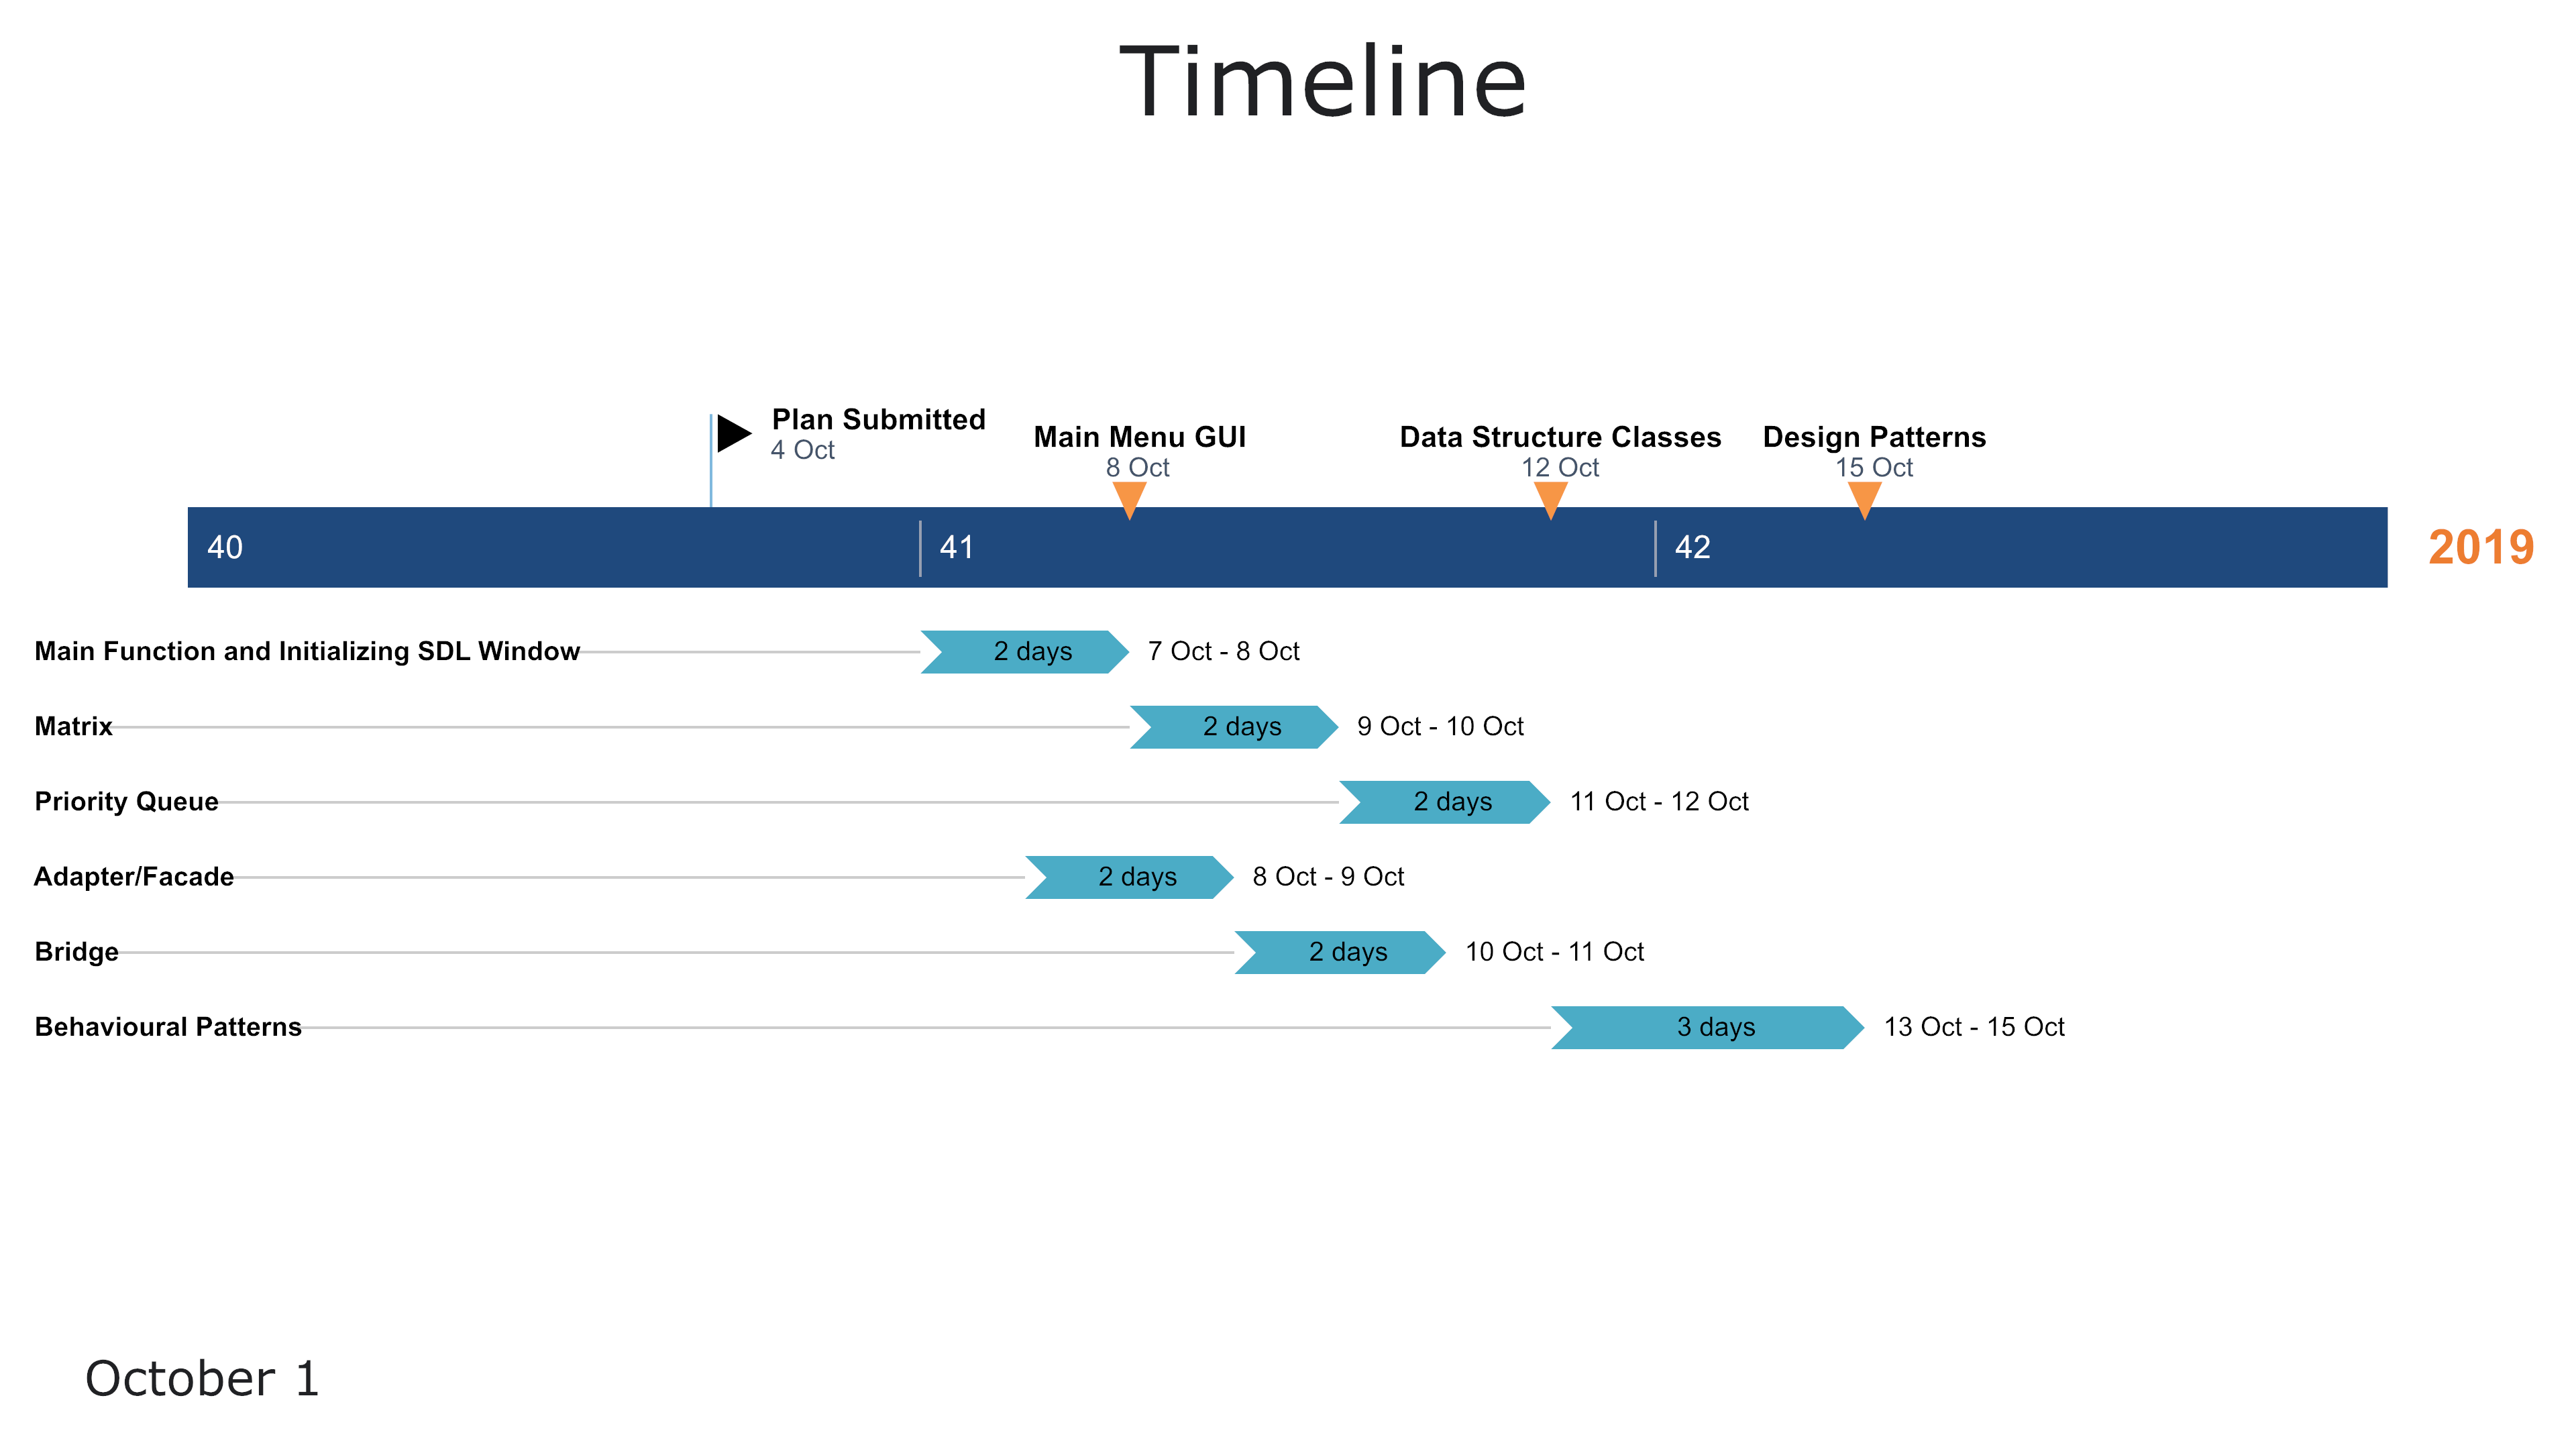
\includegraphics[width=14cm]{October1} 
	}
	\caption{\label{fig:October1} First two Weeks of October.}
\end{figure}

\begin{figure}[h]
	\centering
	\fboxsep 2mm
	\framebox{
		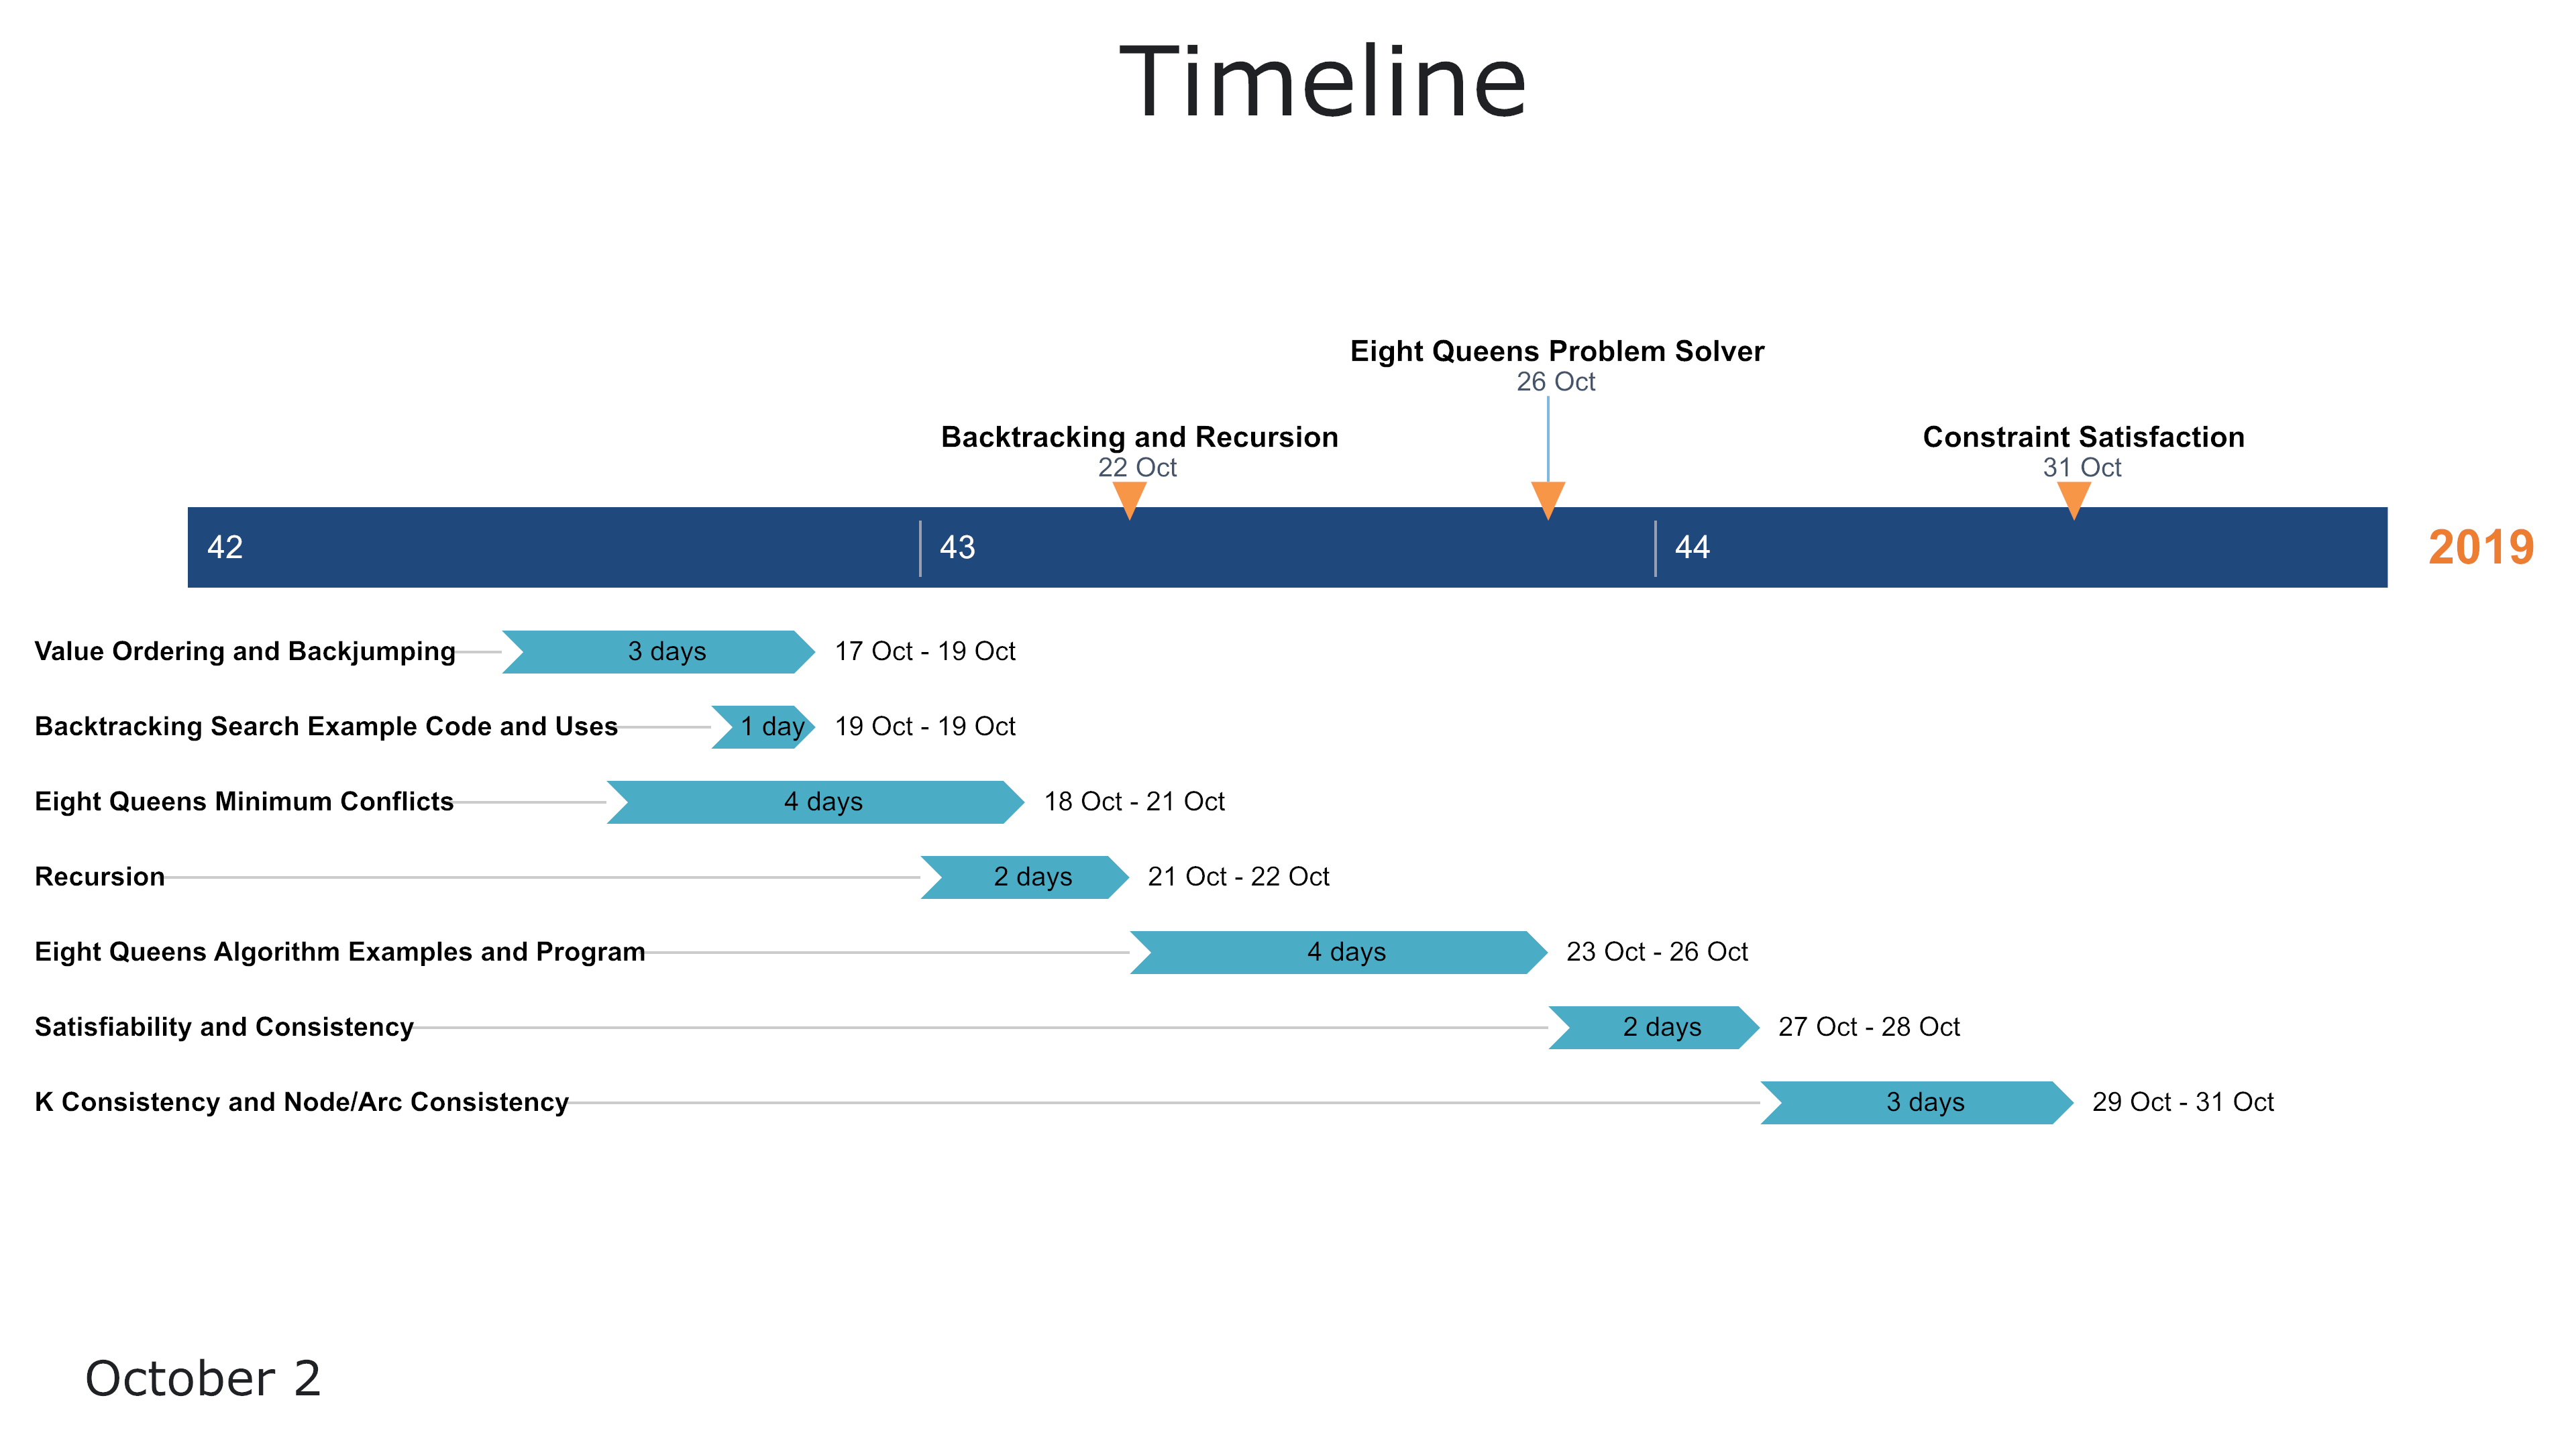
\includegraphics[width=14cm]{October2} 
	}
	\caption{\label{fig:October2} Last two Weeks of October.}
\end{figure}

\begin{figure}[h]
	\centering
	\fboxsep 2mm
	\framebox{
		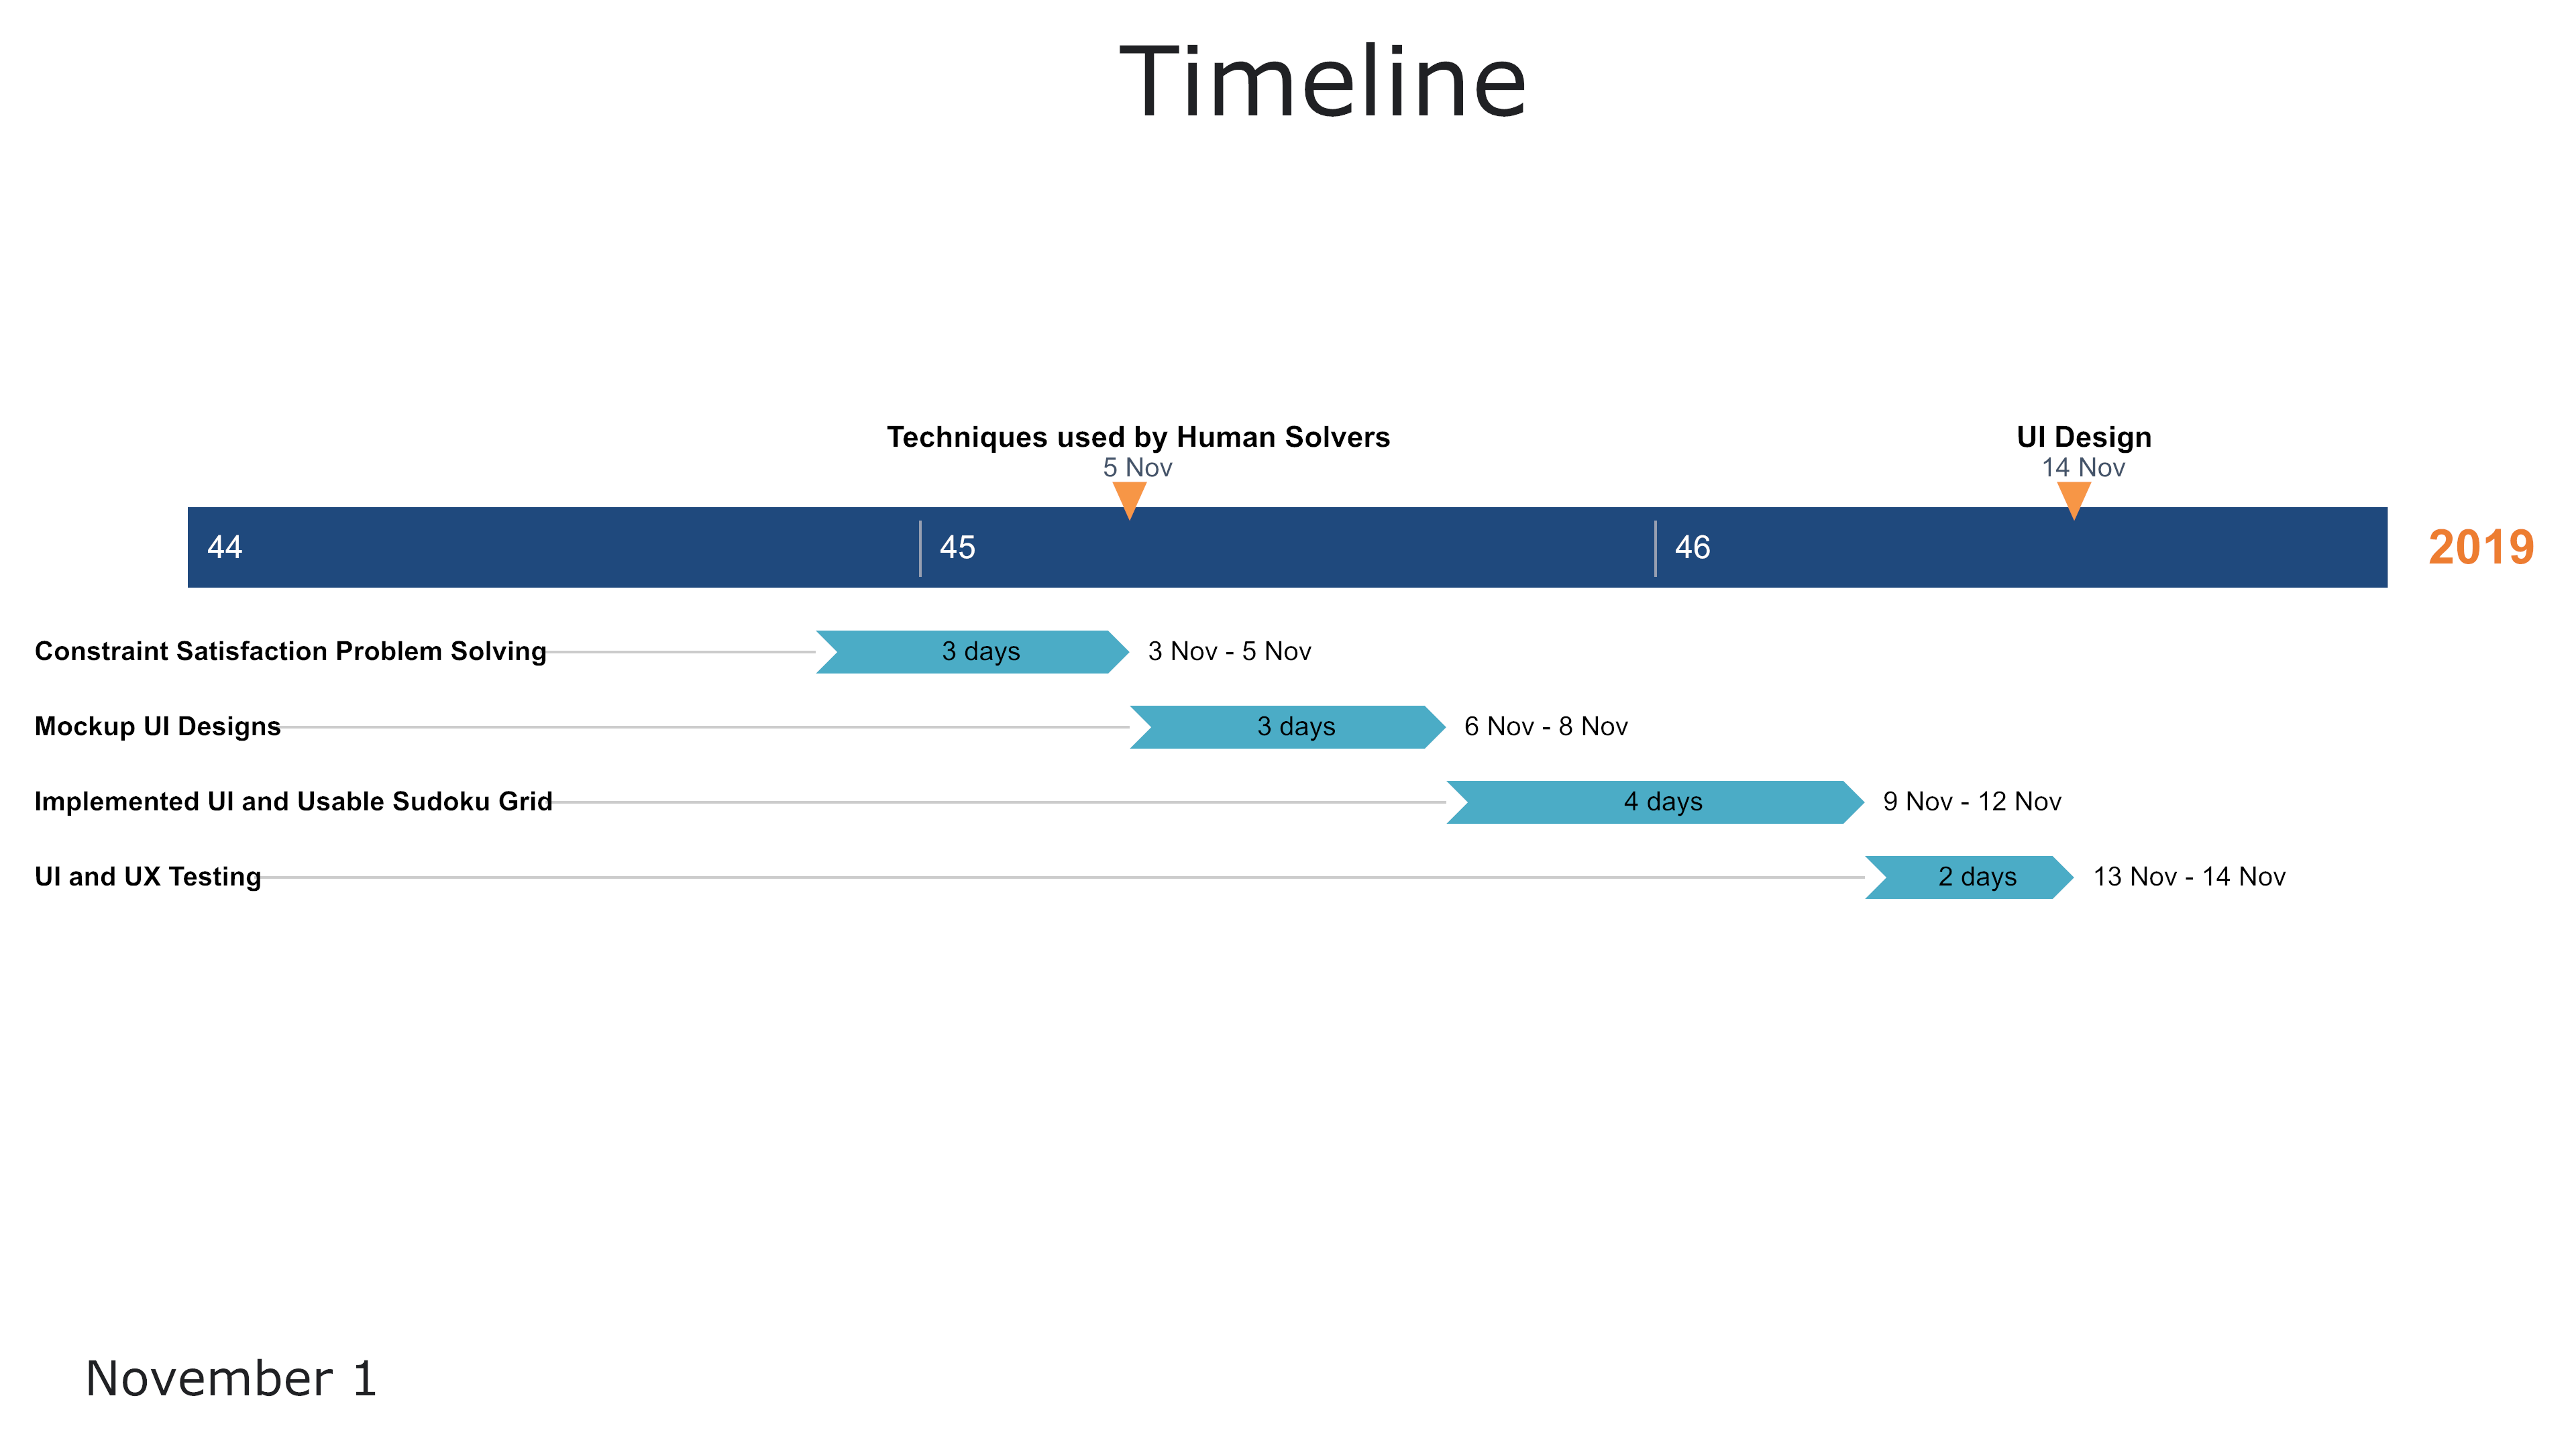
\includegraphics[width=14cm]{November1} 
	}
	\caption{\label{fig:November1} First two Weeks of November.}
\end{figure}

\begin{figure}[h]
	\centering
	\fboxsep 2mm
	\framebox{
		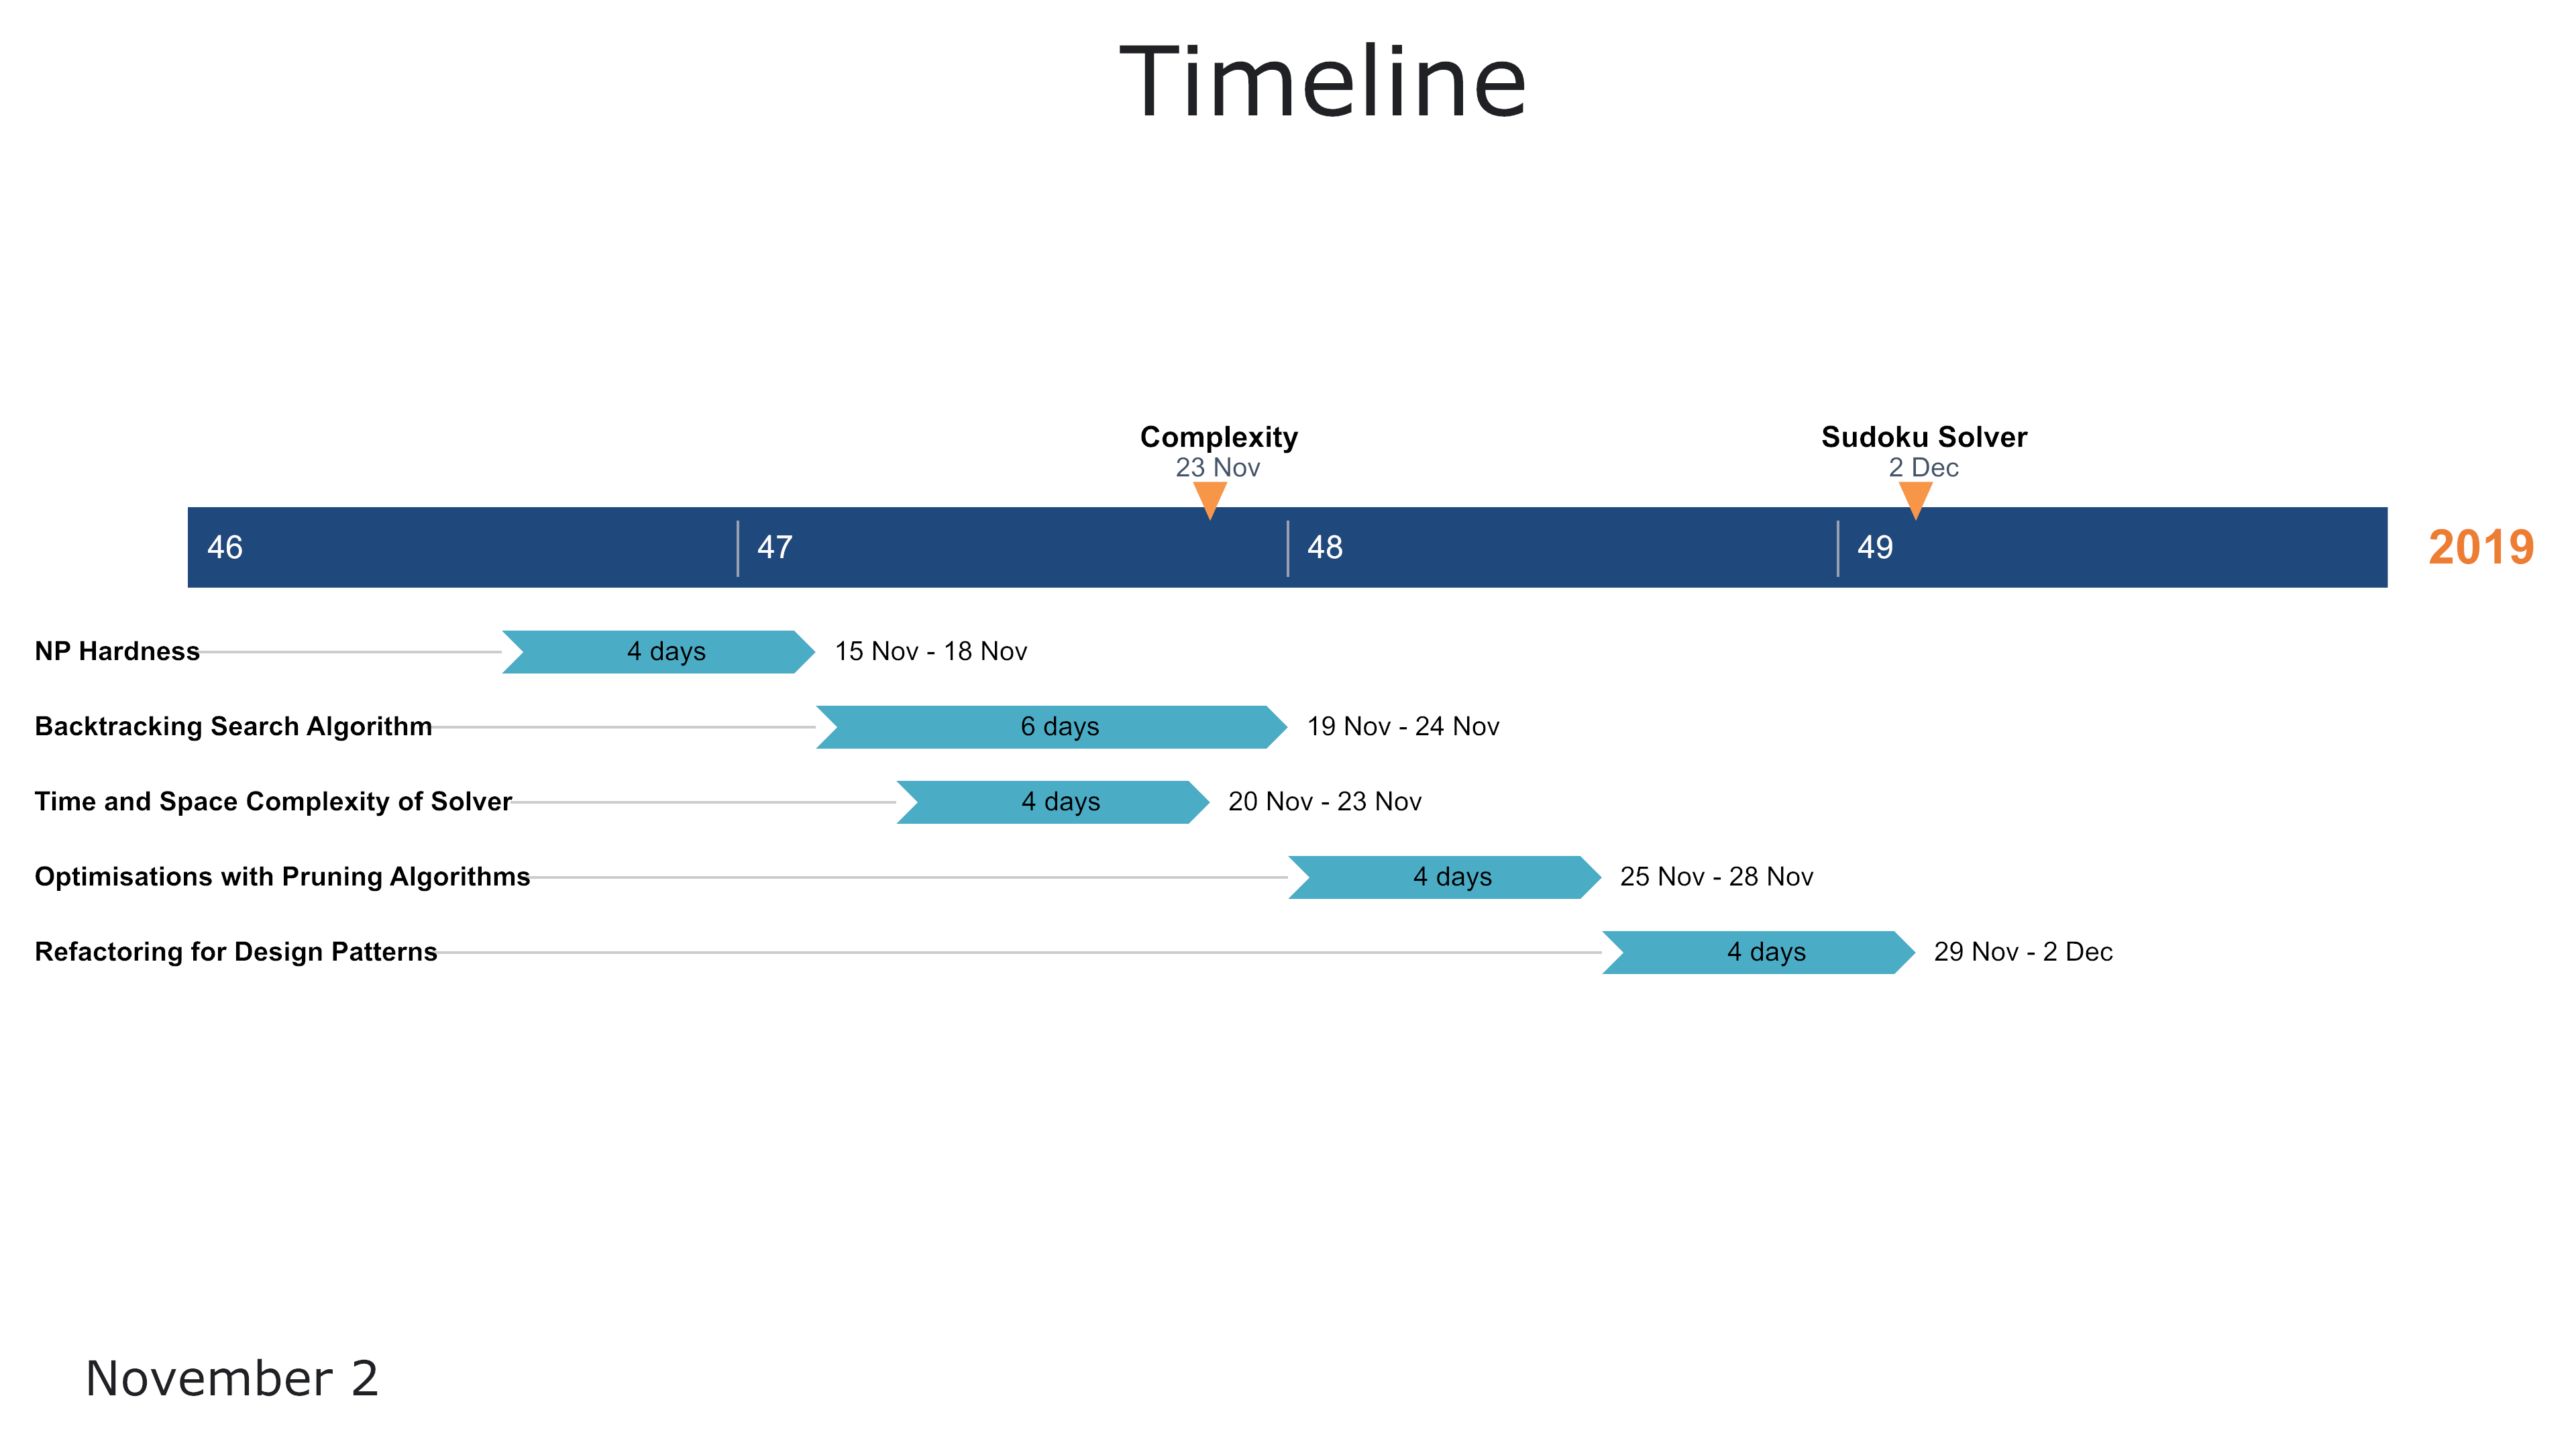
\includegraphics[width=14cm]{November2} 
	}
	\caption{\label{fig:November2} Last two Weeks of November.}
\end{figure}

\begin{figure}[h]
	\centering
	\fboxsep 2mm
	\framebox{
		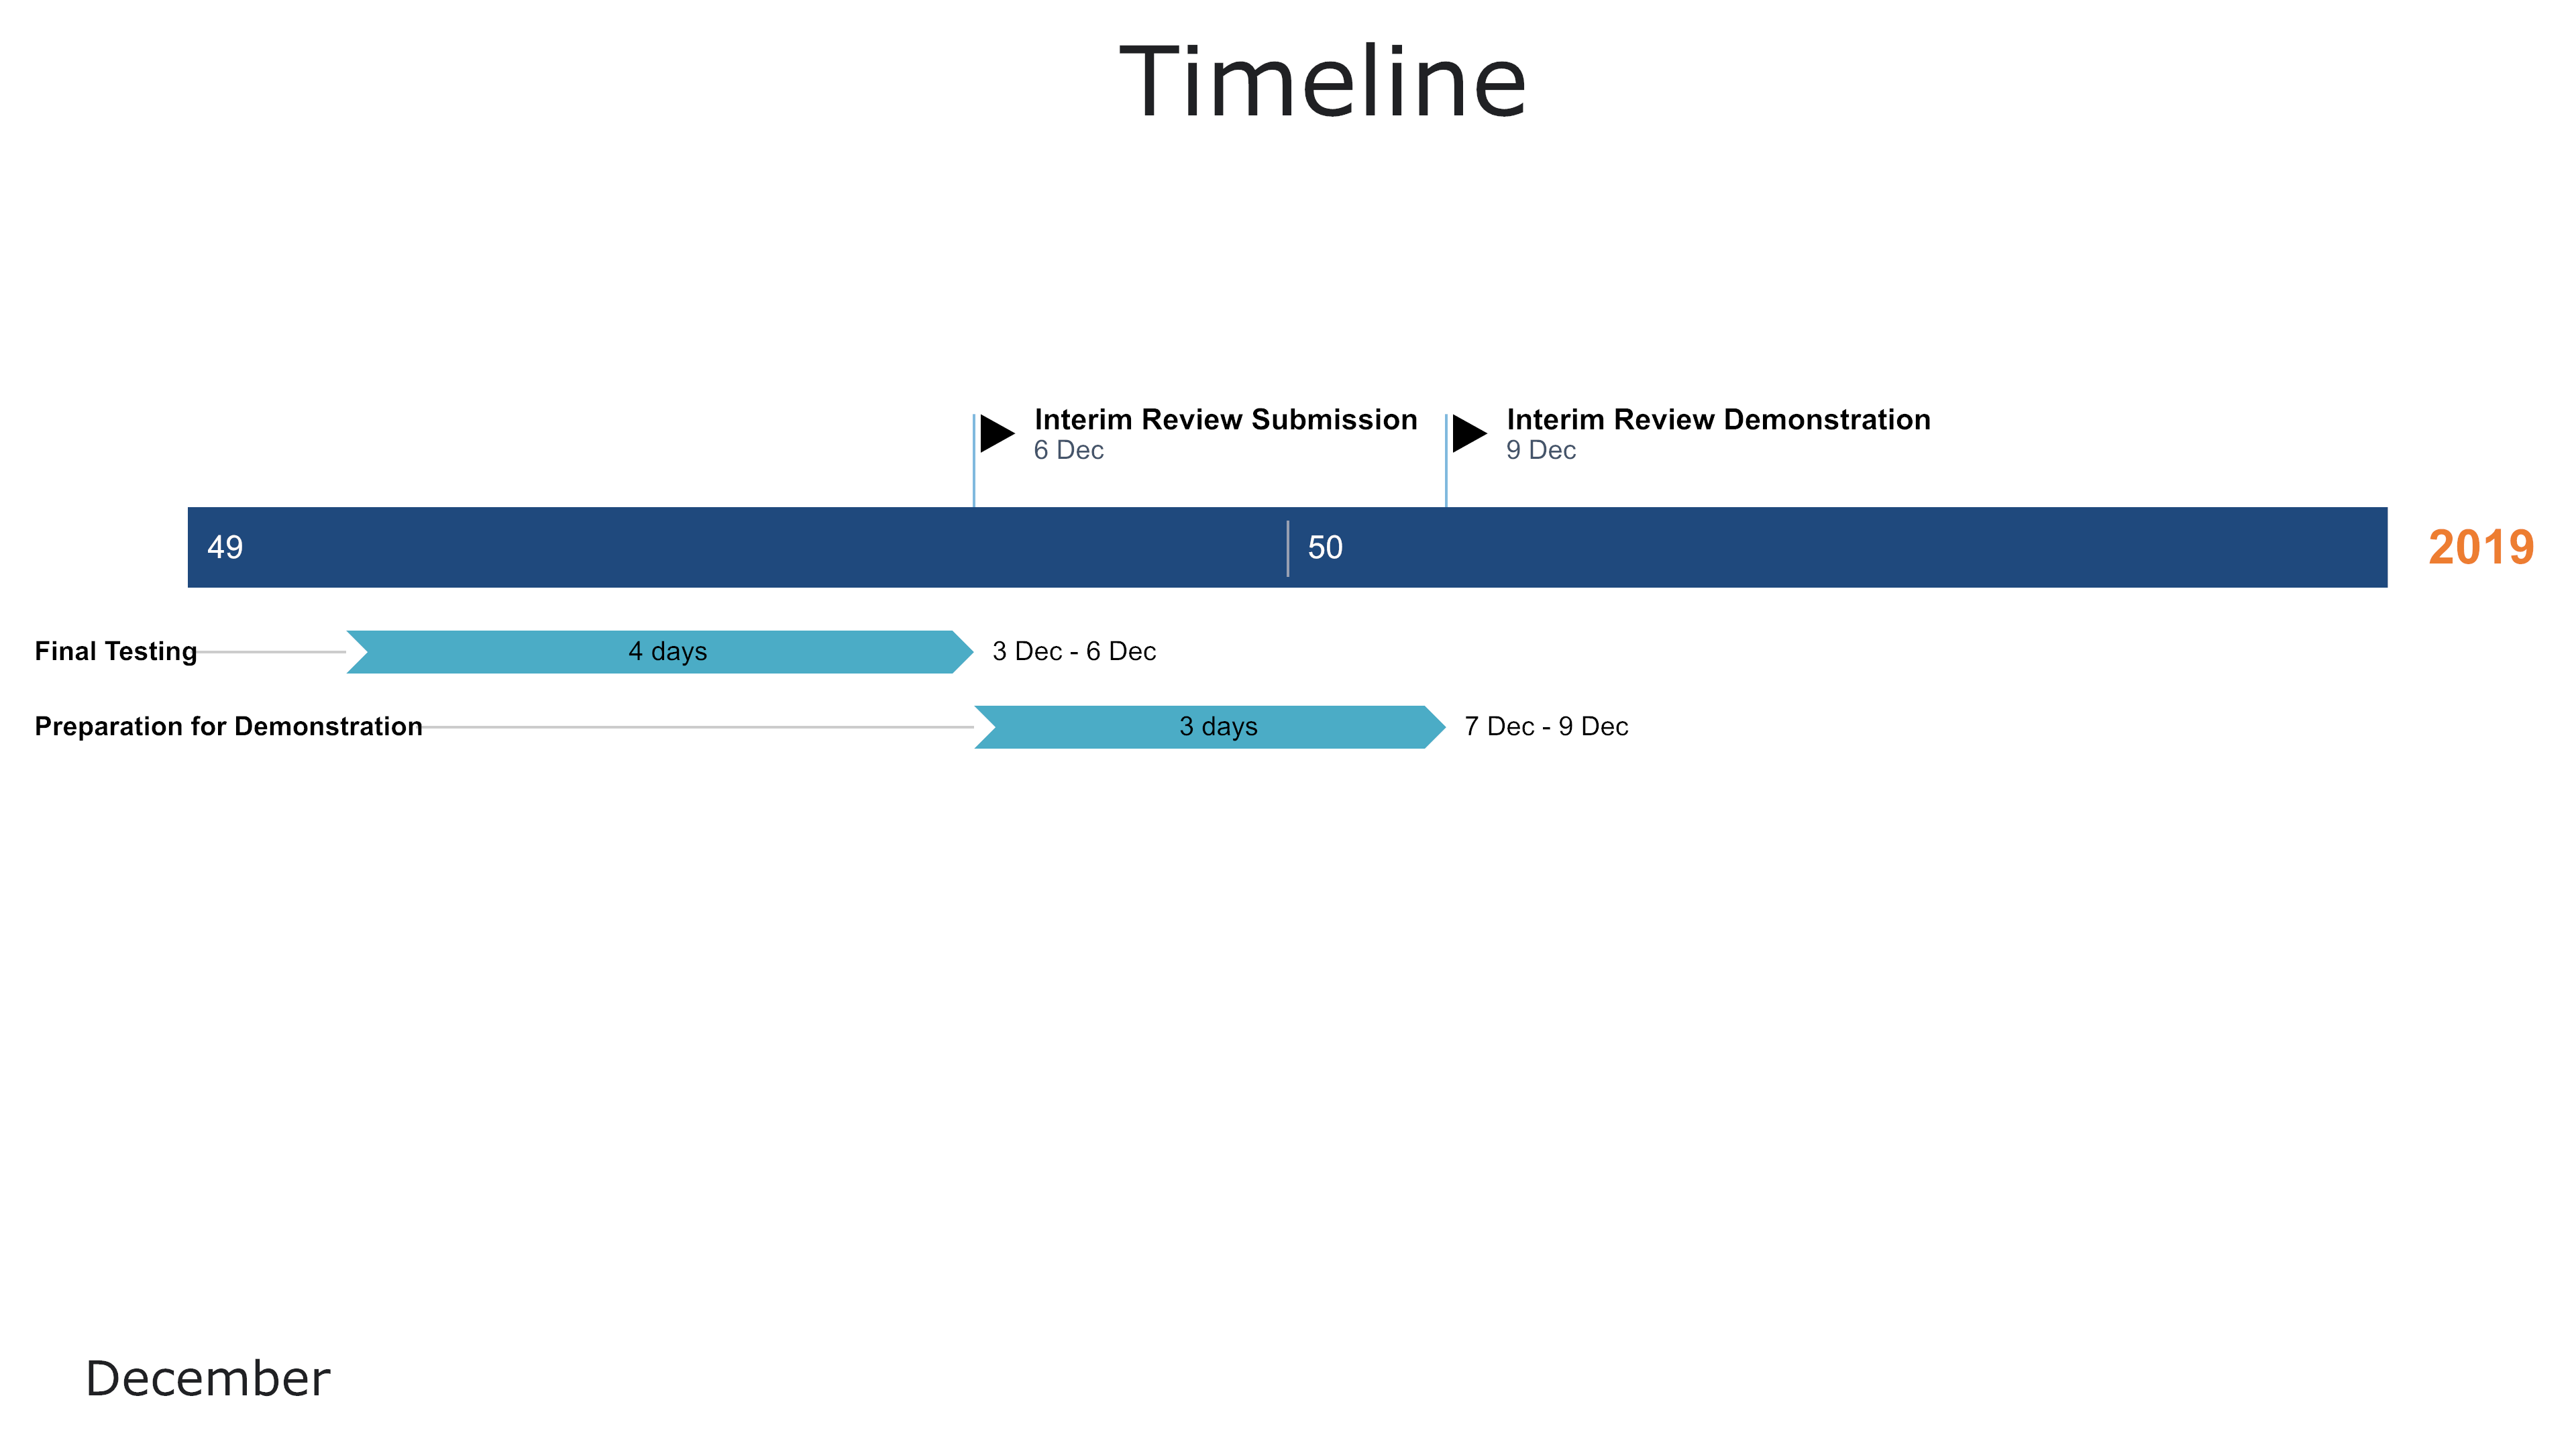
\includegraphics[width=14cm]{December} 
	}
	\caption{\label{fig:December} December.}
\end{figure}

\begin{figure}[h]
	\centering
	\fboxsep 2mm
	\framebox{
		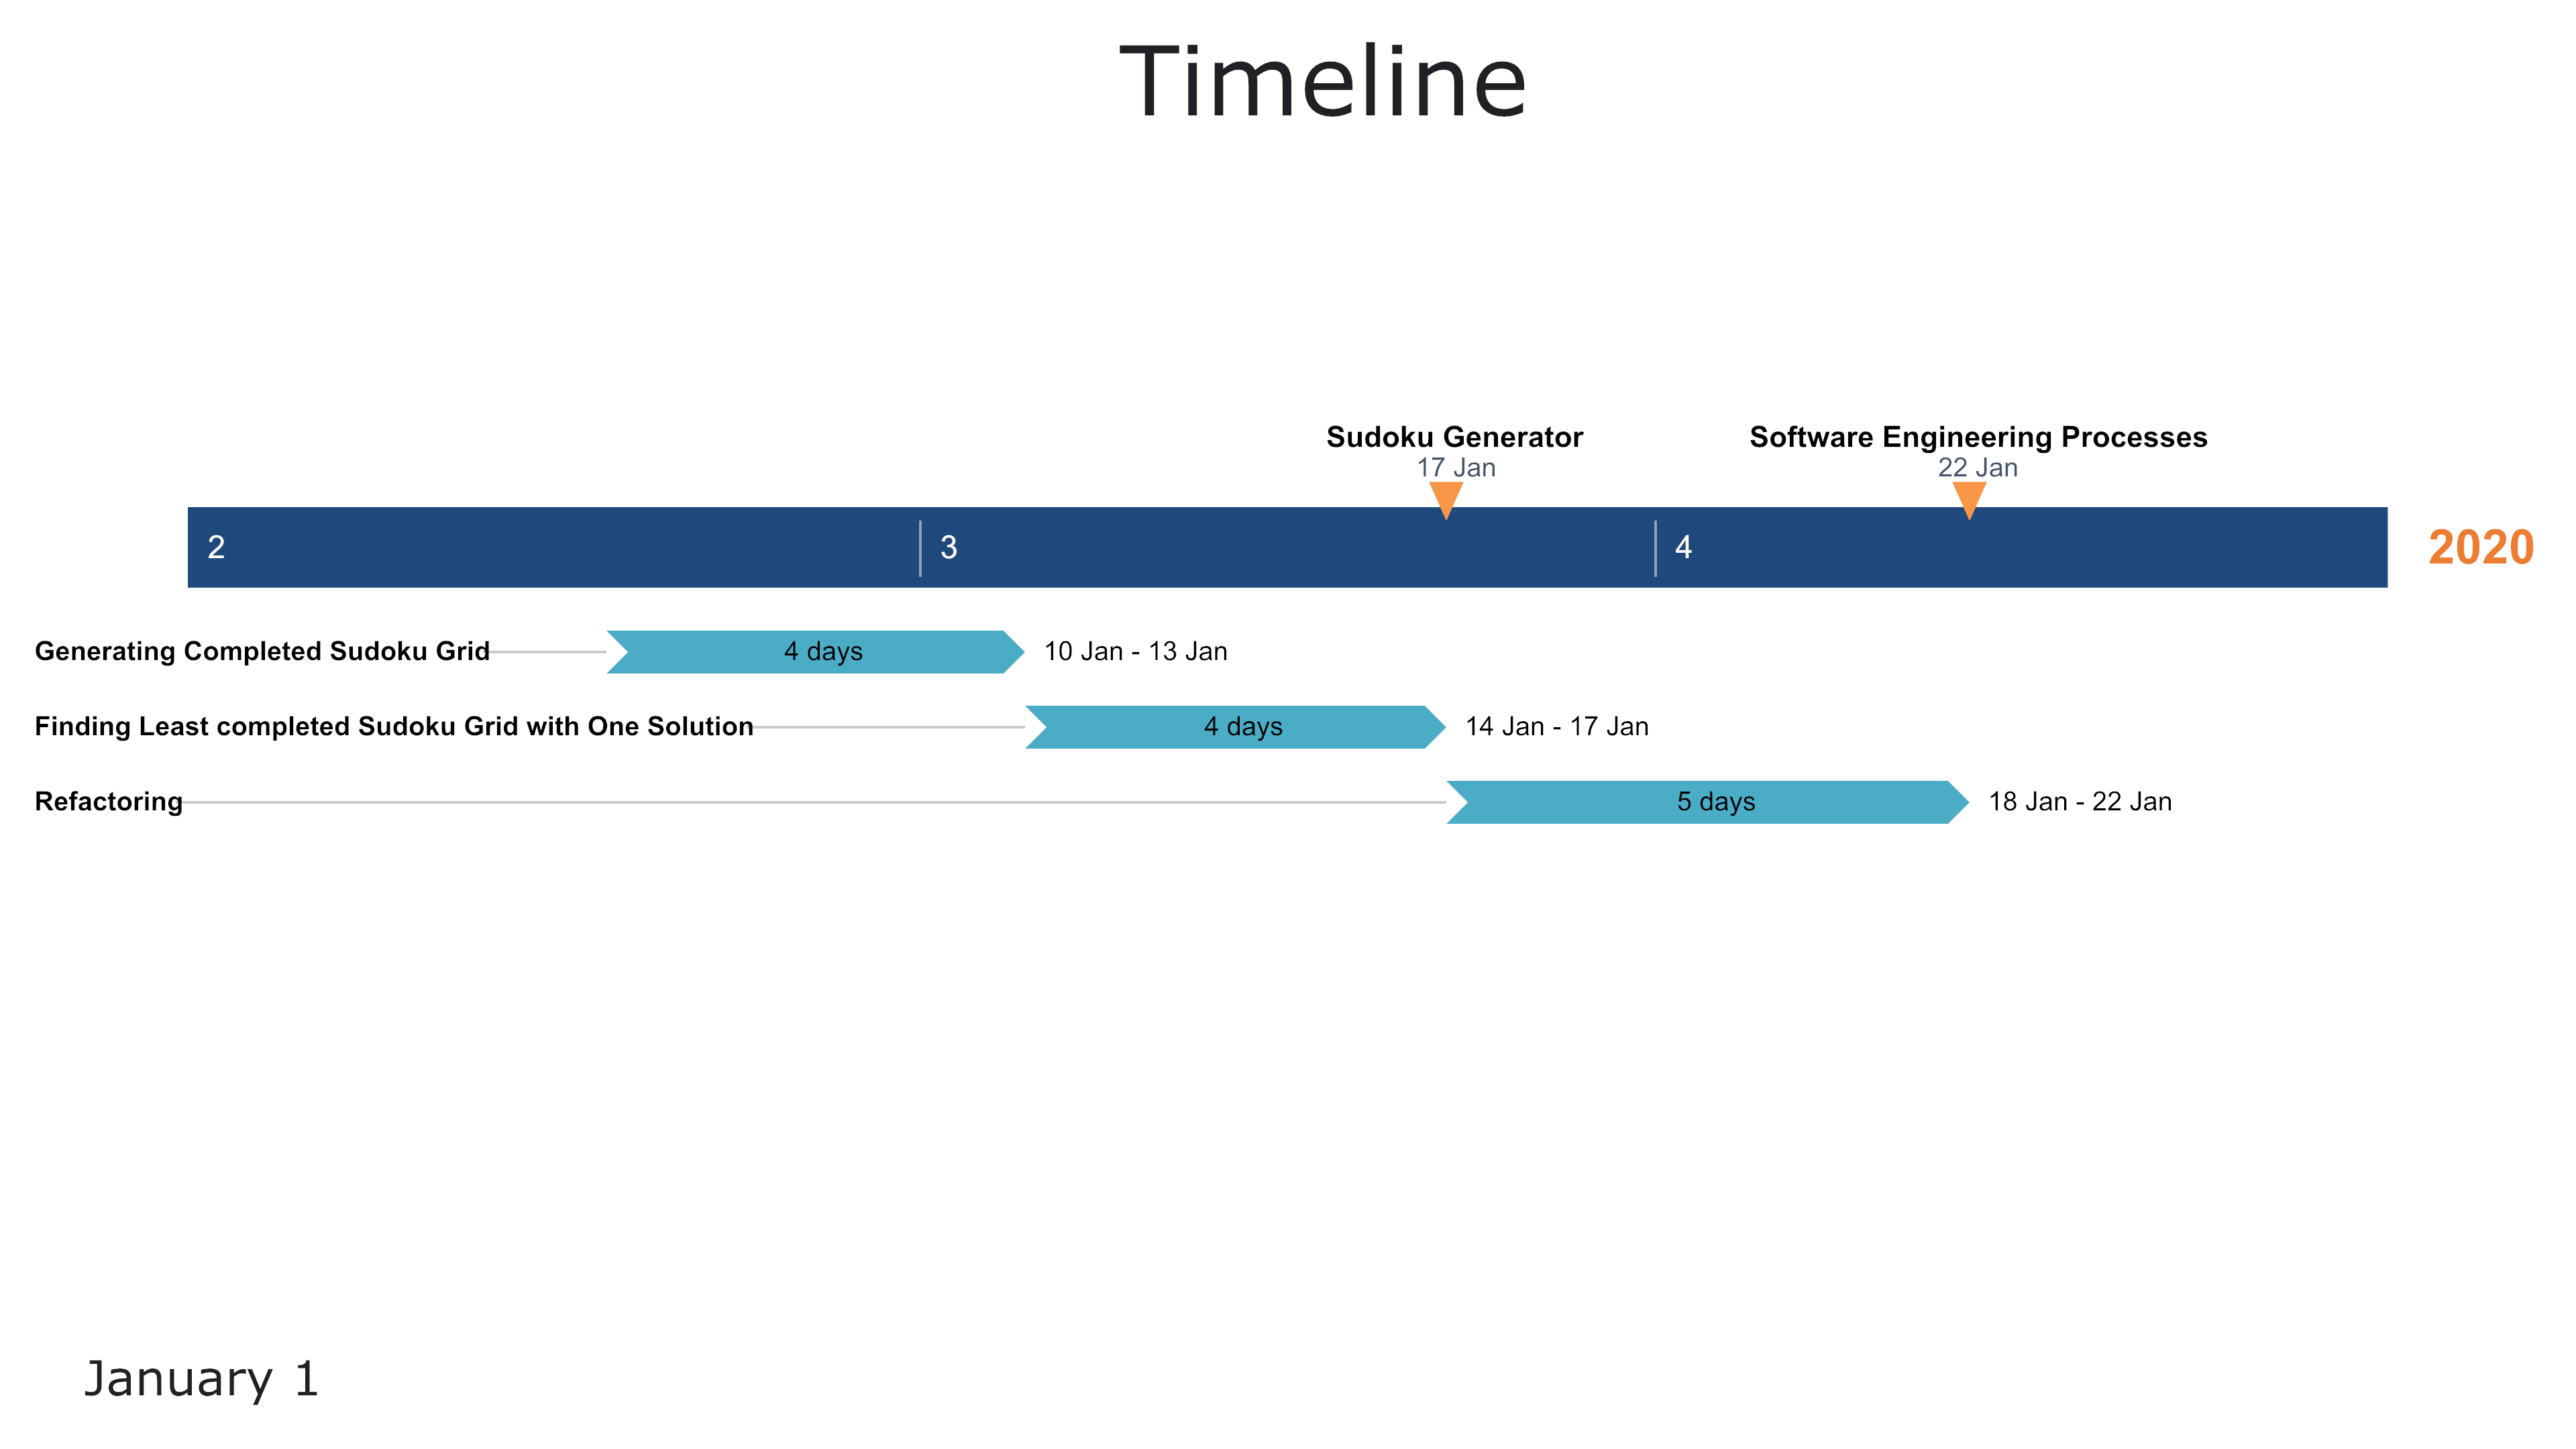
\includegraphics[width=14cm]{January1} 
	}
	\caption{\label{fig:January1} First two Weeks of January.}
\end{figure}

\begin{figure}[h]
	\centering
	\fboxsep 2mm
	\framebox{
		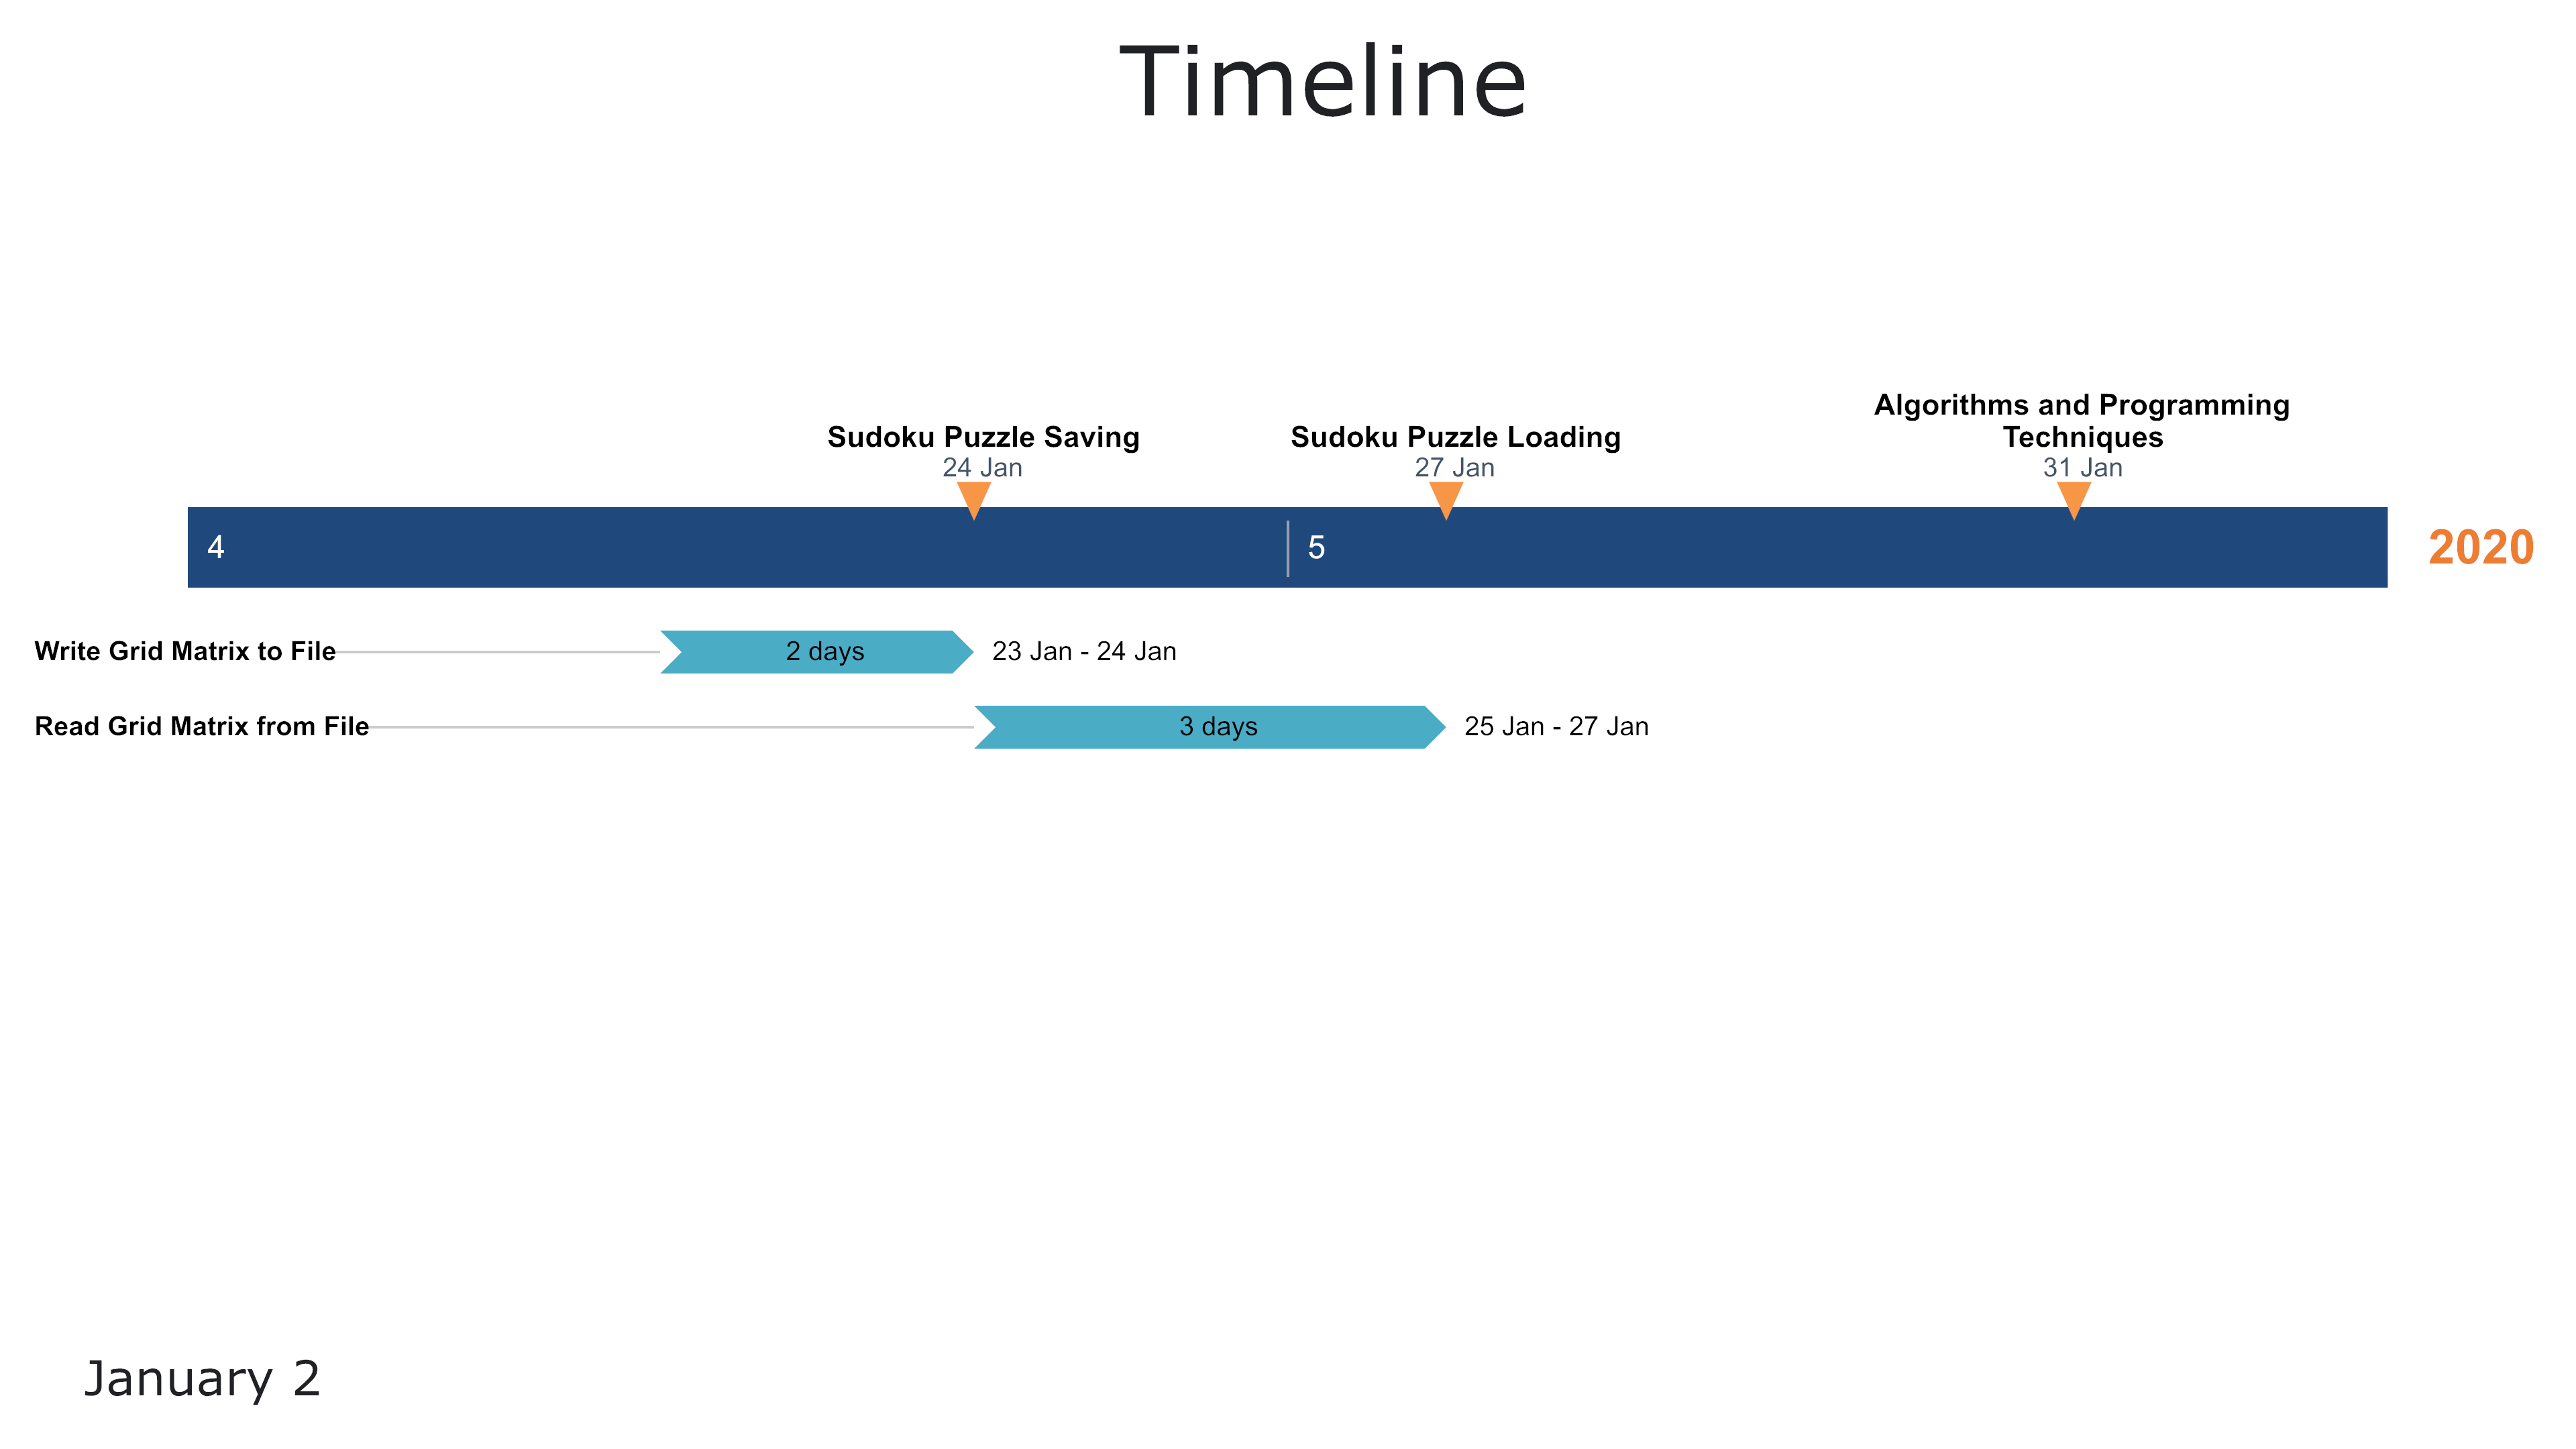
\includegraphics[width=14cm]{January2} 
	}
	\caption{\label{fig:January2} Last two Weeks of January.}
\end{figure}

\begin{figure}[h]
	\centering
	\fboxsep 2mm
	\framebox{
		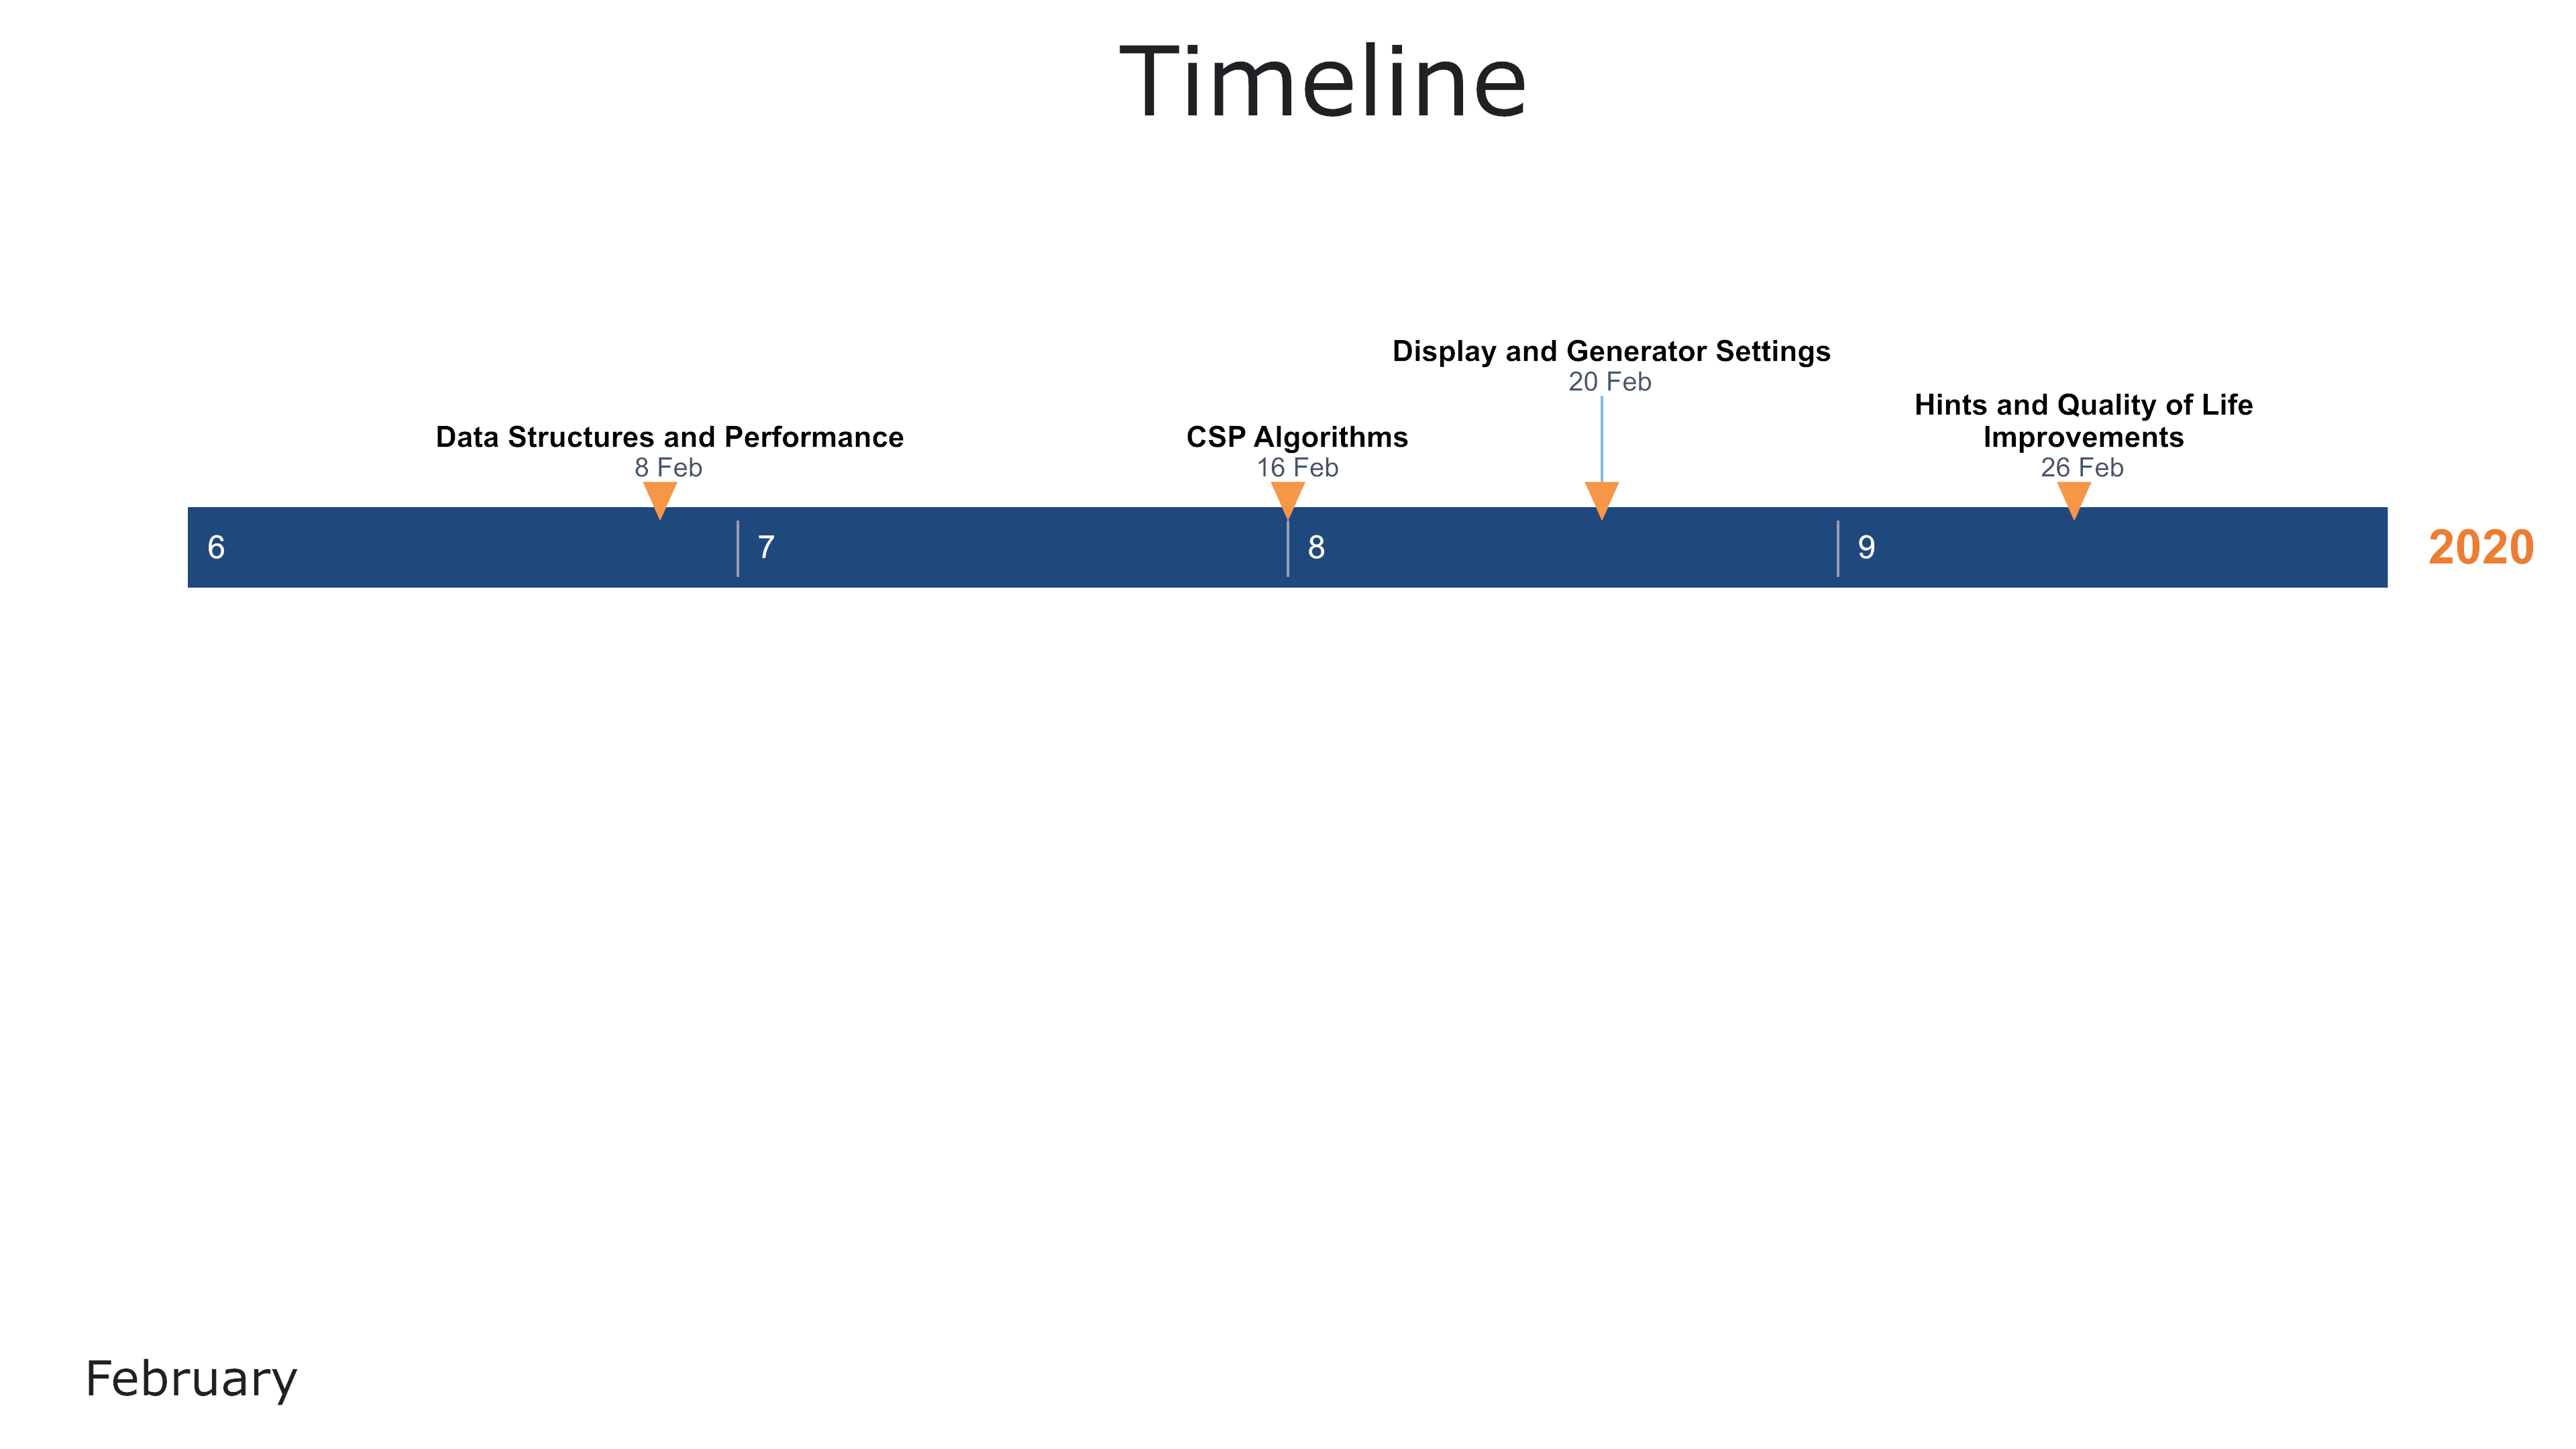
\includegraphics[width=14cm]{February} 
	}
	\caption{\label{fig:February} February.}
\end{figure}

\begin{figure}[h]
	\centering
	\fboxsep 2mm
	\framebox{
		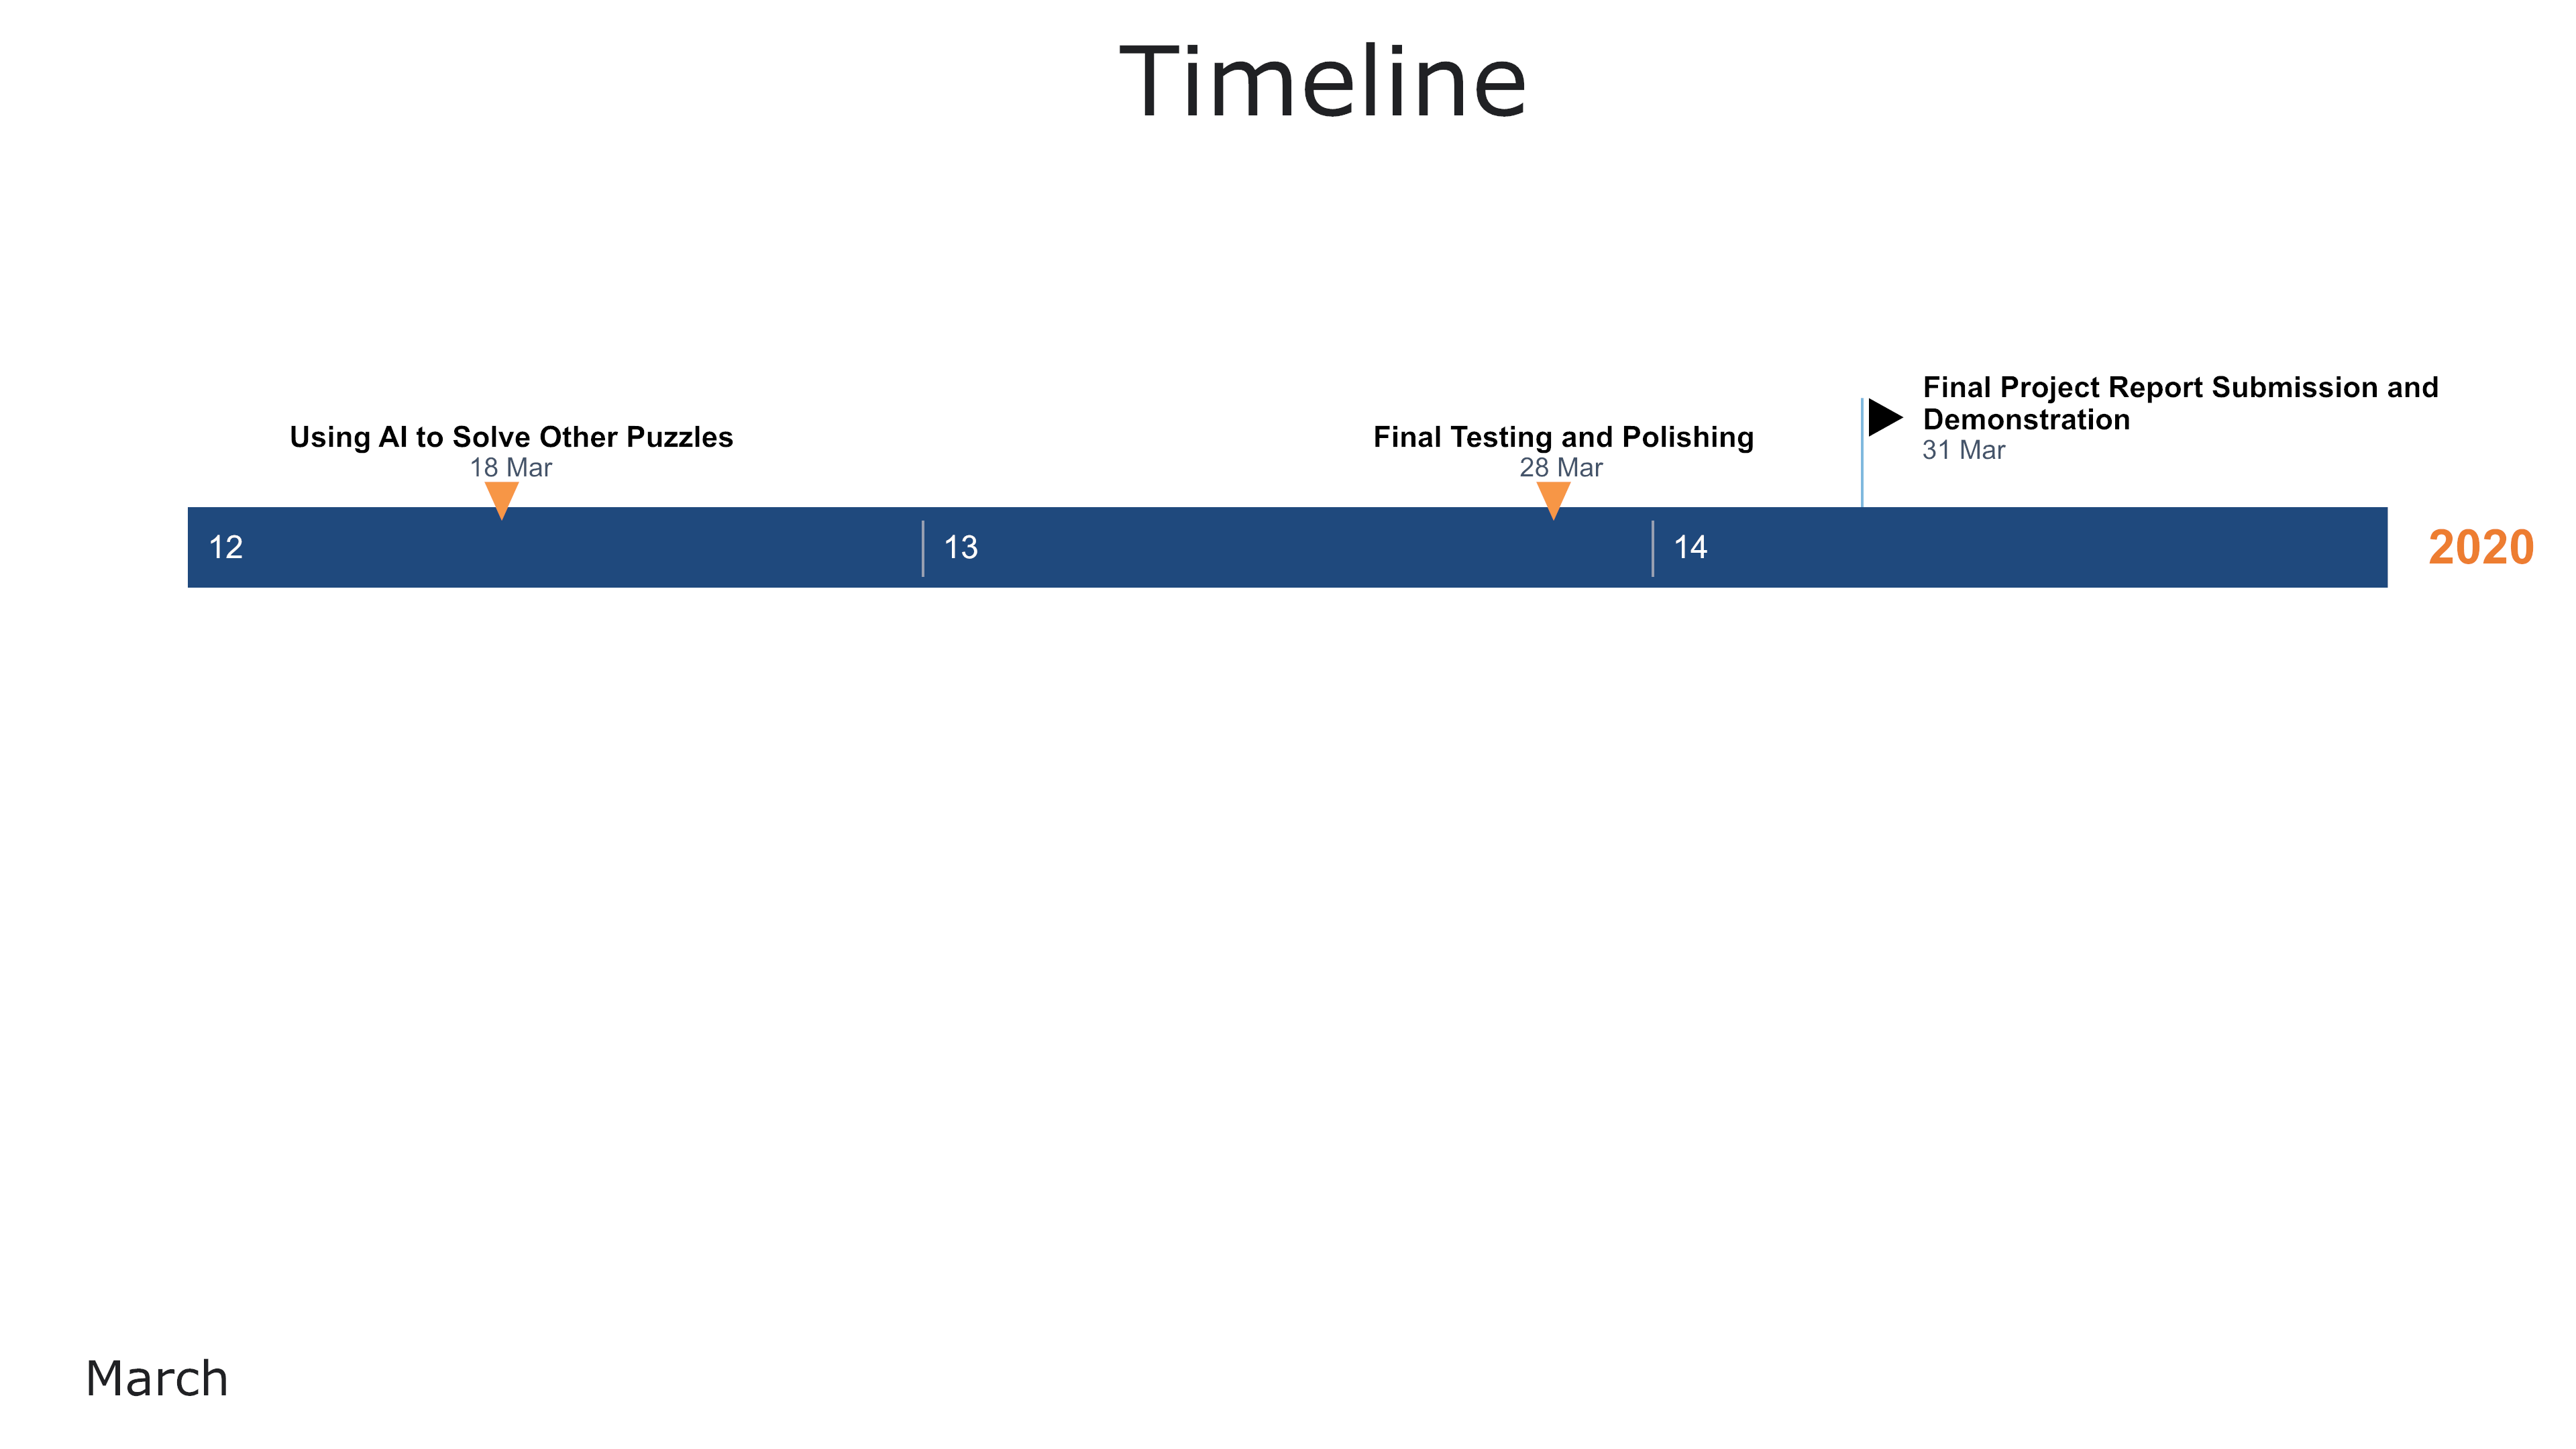
\includegraphics[width=14cm]{March} 
	}
	\caption{\label{fig:March} March.}
\end{figure}

\chapter*{Bibliography}
\addcontentsline{toc}{chapter}{Bibliography}

\section*{Books}
\addcontentsline{toc}{section}{Books}

Foundations of Constraint Satisfaction~\cite{TSANG:1993}

As Sudoku can be described as a Constraint Satisfaction problem, it is relevant to research what these are and how to solve them, this book has detailed explanations and examples that will help in solving the Eight Queens problem and using CSP algorithms.

Artificial Intelligence: A Modern Approach -- Third Edition~\cite{RUSSELL:2016}

This book has relevant information and examples of AI algorithms like backtracking search and efficient algorithms like alpha/beta pruning that will be helpful in generating and solving Sudoku puzzles.

SDL Game Development~\cite{MITCHELL:2013}

As the GUI will be made using SDL 2.0, it is relevant to use this book to see examples of GUI initialisation code and documentation on the framework, which will be helpful in creation the screens to display and solve the Sudoku puzzles.

Design Patterns: Elements of Reusable Object-Oriented Software~\cite{GAMMA:1995}

This books provides a detailed overview of all Design Patterns, which will be relevant when writing about the Software Engineering Processes used in the program and will be helpful in providing examples of how to refactor program code to include Design Patterns.

\section*{Web Pages}
\addcontentsline{toc}{section}{Web Pages}

Solving Every Sudoku Puzzle~\cite{NORVIG:2019}

This website provides useful examples of the backtracking algorithms and how they should work to solve a Sudoku puzzle of any difficulty.

Sudoku Solving Algorithms~\cite{WIKIPEDIA:2019}

This website provides a good overview of different ways of solving a Sudoku puzzle, which could be used to find other more efficient algorithms to use, such as modelling the Sudoku puzzle as an exact cover problem and finding the solution with the dancing links algorithm.

\chapter*{Risk Assessment}
\addcontentsline{toc}{chapter}{Risk Assessment}

The program might not display the GUI as expected or is difficult to configure the GUI window, this is highly likely and important for displaying the Sudoku puzzle to the user, but can be mitigated by making sure that I have read all the documentation for the GUI framework I will be using or switching to another framework if what I want to do is not possible.

I might not be able to generate difficult puzzles to test my AI solving algorithms, this is possible and is important for making sure the solver works correctly, to mitigate this if it happens I will use public domain Sudoku puzzles to test my program.

The program might run slower than expected, making it difficult to test the AI solving algorithms, this is likely and is important as it is one of the objectives of the project, to mitigate this I will research efficient AI solving algorithms like pruning and time implementations of the AI solving algorithms to decide which works best for my program.

The User Interface design and User Experience for the application might be confusing for the user, this is highly likely and will be important for allowing the user to attempt to solve the Sudoku puzzle, I can mitigate the chance of this happening by making good mock up designs of the UI and UX, I can also mitigate this if it does happen by testing different designs using the GUI.

%%%%%%%%%%%%%%%%%%%%%%%%%%%%%%%%%%%%%%

%\begin{verbatim}
%static public void main(String[] args) {
%  try  {
%    UIManager.setLookAndFeel(UIManager.getSystemLookAndFeelClassName());
%  }
%  catch(Exception e) {
%    e.printStackTrace();
%  }
%  new WelcomeApp();
%} 
%\end{verbatim}

\newpage
\begin{thebibliography}{99}
\addcontentsline{toc}{chapter}{Bibliography}
\bibitem{TSANG:1993} Edward Tsang (1993). \emph{Foundations of Constraint Satisfaction}.
\bibitem{RUSSELL:2016} Stuart Russell and Peter Norvig (2016). \emph{Artificial Intelligence: A Modern Approach -- Third Edition}.
\bibitem{MITCHELL:2013} Shaun Mitchell (2013). \emph{SDL Game Development}.
\bibitem{GAMMA:1995} Erich Gamma, Richard Helm, Ralph Johnson and John Vlissides (1995). \emph{Design Patterns: Elements of Reusable Object-Oriented Software}.
\bibitem{NORVIG:2019} Peter Norvig. \emph{norvig.com/sudoku.html}.
\bibitem{WIKIPEDIA:2019} Wikipedia. \emph{en.wikipedia.org/wiki/Sudoku\_solving\_algorithms}.
\end{thebibliography}
\label{endpage}



\end{document}

%\end{article}
